% !TEX program = latexmk
% !TEX encoding = UTF-8 Unicode

% 注意:请使用 TeXLive 2023 及以上版本
% WARNING: Please use TeXLive version >= 2023

% 注意:请确保自己已经完整阅读了 README.md 这一 markdown 文档,部分功能的使用方法并未在 .tex 中直接给出;如果仍有使用问题,请在 Github 上提出 issue
% WARNING: Pleans read README.md first cause some usages are not given in .tex files.

%%%%%%%%%%%%%%%%%%%%%%%%%%%%%%%%%%%%%%%%%%%%%%%%%%%%%%%%%%%%%%%%%%%%%%%%%%%%%%%%%%%%%%%%%%%%%%%%%%%%%
%% select the basic style of this thesis/dissertation (this document will use thesis for convenience)
%% 选择论文的基本类型

\documentclass[
    master,     % 必选项:   {master, doctor} 此处不区分专业/学术学位,在下面学位类型处区分
                % Mandatory: {master, doctor} No difference between Academic degree and Professional degree,
                %                             but be careful about arguments in `\degree' and `\subject'
    % english,  % 可选项:   英文正文请选择此项
                % Optional:  For english main content, It will change some auto-generated matter into English
    % blind,    % 可选项:   论文用于盲审请选择此项,将隐去致谢页内容(但保留标题)、答辩委员会会议决议页内容(同前)、
                %            常规评阅人名单页内容(同前),将隐去题名页、答辩委员会页所有人名,
                %            注意:如果非自动读取成果数据库,请自行修改 `攻读学位期间取得的研究成果' 内的内容格式
                % Optional:  For blind review, It will not generate Acknowledgements(Content), Decision of Defense
                %            Committee(Content), General Reviewers List(Content), hide all names.
                %            NOTICE: CHANGE THE STYLE of Achievements BY YOURSELF
    % plgck,    % 可选项:   论文用于查重请选择此项,将只产生从摘要到附录(含)的内容,且所有图片均不显示
                % Optional:  For plagiarism check, It will only produce content from abstract to appendicies, 
                %            meanwhile all figures will not be displayed.
]{XJTU-thesis}



%%%%%%%%%%%%%%%%%%%%%%%%%%%%%%%%%%%%%%%%%%%%%%%%%
%% fill the each blank for auto-generate contents
%% 填写以下信息用以自动生成

% 论文标题(不超过35个字,英文注意大小写规律)
% Title, Make sure you have an acceptable capitalization
\title{用于脑卒中快速鉴别的生成式EIT图像重建算法的研究}{Research on Generative EIT Image Reconstruction Algorithm for Fast Detection of Stroke}

% 学位类型
% 考虑到专业学位的学位名称的少数特例(如专业型法学硕士不是 Master of Juris 而是 Juris Master),此处学位类型请按照案例和文件填写
% 同时为了前向兼容,可选项「A/P」(实际必须正确选择)代表「学术/专业」型学位,默认为学术型
% Type of your degree, Translate it from documents in `Materials/Requirements/2021/01 中英文题名页示例/英文标准翻译/'
% \degree[A]{硕士}{Master of Engineering} % 学术型(Academic)硕士请基于 '学术学位名称.txt' 填写
% \degree[P]{工程硕士}{Master of Engineering} % 专业型(Professional)硕士请基于 '专业学位(领域)英文标准翻译.pdf' 填写
%\degree[A]{博士}{Doctor of Philosophy}  % 学术型(Academic Doc)博士请填写 '{博士}{Philosophy}'
\degree[P]{工程硕士}{Master of Engineering} % 专业型(Professional Doc)博士请基于 '专业学位(领域)英文标准翻译.pdf' 填写

% 作者姓名(注意:所有人名英文均为「名在前,姓在后」,如果只有外文名,请在两个参数都填写外文名称)
% If you have only foreign name, put it as both first and second argument
\author{张里园}{Liyuan Zhang}

% 指导老师姓名(注意:同作者姓名)
% Name of supervisor, It have the same requirments as the author
\advisor{金莉\quad}{副教授}{Li Jin}{Prof.}

% 合作指导老师姓名 或 老师团队(合作指导老师指:1.与招生简章中一致的合作导师,2.CSC项目的合作导师)
%(校方模板要求只能选择一个,都有则显示合作导师)
% Name of associate advisor or adviror's team, You can use only one of them, and advisorassociate has a higher priority.
% \advisorassociate{陈尘}{副教授}{Chen Chen}{Asscociate Prof.}
% \advisorteam{团队中文名}{English Name of the Team}

% 学科名称,请基于 '学科(专业)英文标准翻译.pdf' 填写
% Name of the subject, also get it from that file
% \subject{航空宇航科学与技术}{Aeronautical and Astronautical Science and Technology}
\subject{电子信息}{Electrical Information}

% 论文提交日期,不输入参数则默认使用当前日期,如手动指明年月,请在第一个可选参数内填写年份,第二个可选参数填写月份(均为阿拉伯数字)
% Submission date of this thesis, if you not put it manually, it will use the current time
% \submitdate[2021][06]
\submitdate

% 答辩委员会委员 显示的顺序和这里的一样 第一个人是主席
% Committee member of your defence, notice that the order shows in the thesis is same as here, and the first one is the chairperson
% each member should be put as {Organization,Name,Title} split by comma
\addcommitteemember{西安交通大学,张长长,教授}
\addcommitteemember{西安理工大学,王旺旺,教授}
\addcommitteemember{国网陕西经济技术研究院,李力,高工}
\addcommitteemember{西安交通大学,东方不败,副教授}
\addcommitteemember{西安交通大学,赵照,研究员}

% 答辩时间(手动指定)
% Defence date, input manually
\defensedate{2021}{06}{22}

% 答辩地点(涉密论文请手动设置为「西安交通大学」)
% Defence location, default value is 「西安交通大学」
\defenseloc{西安交通大学主楼E座303室}

% 常规审阅人 要求和答辩委员会委员一样
% General reviewer list, same requirements as the committee member
\addgeneralreviewer{西安交通大学,张长长,教授}
\addgeneralreviewer{西安理工大学,王旺旺,教授}
\addgeneralreviewer{国网陕西经济技术研究院,李力,高工}
\addgeneralreviewer{西安交通大学,东方不败,副教授}
\addgeneralreviewer{西安交通大学,赵照,研究员}

% 学院
% School or Faculty, unused now
% \school{电气工程学院}{School of Electrical Engineering}

% 专业[学士学位使用]
% Major, unused now
% \stumajor{计算机科学与计数}{Computer Science}

% 学号[学士学位使用]
% Student ID, unused now
% \stuid{}

% 班级[学士学位使用]
% Administrative class, unused now
% \adminclass{电气7xx班}{}

% 参考文献源 参数中不要添加 .bib
% 请使用 \addreferenceresource 添加数据库(可导入多个参考文献数据库)
% 若自动化导入攻读学位期间的成果则使用 \addachivementresource
\addreferenceresource{References/reference}
\addachivementresource{References/achievement}

%%%%%%%%%%%%%%%%%%%%%%%%%%%%%%%%%%%%%%%%%%%%
%% 如果有使用其他包,请在这里添加
%% If you need other packages, use them here

% \usepackage{}


%%%%%%%%%%%%%%%%%%%%%%%%%%%%%%%%%%%%%%%%%%%%%%%%%%%%%%%%%%%%%%%%%%%%%%%%%%%%%%%%%%%
%% 注意:根据校方要求,以下所有页面顺序不可调整
%% Notice: The order of these pages are defined in the requirements of the University.

%% 但在最终提交前,可以通过注释所有 \thesis 开始的命令设置是否生成各个部分
%% 或根据说明调整 latexmkrc 文件,使用 \includeonly 命令导入部分章节。

% \includeonly{
%   Main_Spine/c1,
%   Main_Spine/c2,
%   Main_Spine/c3,
%   Main_Spine/c4,
%   Main_Spine/c5,
%   Main_Spine/c6,
% }

\begin{document}
% [自动生成] 中英题名页
% [Auto Generate] Chinese English Title Page
\thesistitles

% [自动生成] 答辩委员会页
% [Auto Generate] Defense Committee Pages
\thesiscommittes

% 生成摘要页 修改 Main_Miscellaneous/abstract_chs/eng.tex 中的内容
% Abstract, Rewrite your content in Main_Miscellaneous/abstract_chs/eng.tex
\thesisabstract

% [自动生成] 中英目录页
% [Auto Generate] Table of Contents
\thesistableofcontens

% 主要符号表 修改 Main_Miscellaneous/glossary.tex 中的内容
% Glossaries Page, Rewrite your content in Main_Miscellaneous/glossary.tex
\thesisglossarylist

% 正文 使用 \thesisbodybegin & \include & \thesisbodyend 组合导入正文
\thesisbodybegin
% !TeX root = ../main.tex

\xchapter{绪论}{Introductions}

\xsection{研究背景和意义}{Backgrounds}

脑卒中是世界第二大致命的疾病,俗称为中风,除了高死亡率外,幸存者也可能会失去
视力、语言、瘫痪或神志不清。全世界每年有约 1500 万人患中风。其中 500 万人死亡,另
有 500 万人终身残疾,这严重危害到患者的健康,并且给家庭和社区造成了严重的负担。
因此,及时的治疗对于脑卒中的患者而言至关重要。通常而言,脑卒中由致病原因不同可分为两种类型,即
出血性脑卒中和缺血性脑卒中。缺血性脑卒中通常由于血栓阻塞了大脑部分的血液供应
而导致,出血性脑卒中则是由于脑中血管破裂引起的脑出血所导致。因此不同类型的脑
卒中所对应的治疗的手段有所不同。其中缺血性卒中通常可以利用溶栓剂(thrombolytic)治
疗;而出血性卒中则可通过血管内手术使其康复。同时,利用药物治疗缺血性脑卒中的有效
治疗时间通常在四个半小时内。由此可见,实现院前的脑卒中快速检测和类型诊断并展开救治,
能够降低脑卒中的致死致残率。

随着生物医学的飞速发展,各种先进的技术在医学成像中得到更加广泛应用。目前卒中
最主要的鉴别手段即是利用医学成像技术如 X-CT 所得到的结果进行判断。除此之外,医学
成像技术对于其他临床疾病的诊断和治疗有着巨大的意义,已成为临床诊断与医学研究中不
可或缺的一部分。计算机断层扫描(Computed Tomography, CT)作为过程层析成像
(Process Tomography, PT)的一种, 通过利用物理介质与人体发生相互作用来计算出其断层
图像,从而直观的呈现出人体组织器官的形态。目前国内外用于临床诊断的 CT 技术主包括
X 射线计算机断层扫描成像(X-ray computed tomography, X-CT)、超声层析成像(Ultrasound
Tomography)以及磁共振成像(Magnetic Resonance Imaging, MRI)等。在这些 CT 诊断技
术中,X-CT 的成像精度高,但是由于X射线的辐射对人体有害,因此在很多情况下不适于
大量重复使用,甚至不能对特定的群体使用(对于孕妇等)。超声CT利用超声波反射的信息
重建出人体内部的图像,是目前最安全的 CT 技术。但是由于难以建立超声波在人体内部吸
收、投射和反射的确定关系,目前的超声波成像技术忽略了超声波与人体组织之间的相互作
用而得不到理想的定量结果。MRI 可以提供分子水平的信息,能够发现人体生理化学的早期
变化,但是该技术成像速度较慢并且观察不到骨组织信息。
上述传统的 CT 诊断技术在临床上应用广泛,都能获得清晰的人体组织图像,但在医疗
实践中不尽如人意之处在于其成像成本高,价格昂贵、设备复杂并且对使用场景有一定的限
制,也不便于连续监测。对于卒中这类发病快、死亡率高的疾病而言,传统的 X-CT 由于设
备复杂庞大而无法实现及时的院前检测。因此人们迫切需要一种能够避免上述一部分缺陷从而
适用于院前脑卒中类型鉴别诊断的医学成像技术,
电阻抗成像(Electrical Impedance Tomography, EIT)技术就是其中之一。

EIT技术是一种无创、实时、可便捷化的新型医学成像技术。该技术通过向未知场内注入激励电流并测量场域边界的电压分布
从而重建出其内部电导率分布的图像。根据生物电化学理论可以知道,人体内不同组织的电导率(电阻率)不同(\cref{table:table1} 列出了人体主要组织和器官的阻抗分布,可以看到组织器官含水量和电导率
成正比),且同一组织不同健康状况下的电导率也不同(\cref{table:table2} 给出了大脑在不同病变状态下的阻抗变
化),这种差异性为 EIT 的技术的实现提供了生物医学基础。
对于脑卒中类型鉴别而言,由于缺血性脑卒中和出血性脑卒中所对应病灶区域的含水量有显著差异,因而患者颅内的阻抗分布应同样具有显著差异。
因此EIT能通过重构出脑卒中病灶组织的电导率从而区分其类型。

\begin{table}[H]
  \center
  \caption{20~100kHZ 下人体部分器官组织的阻抗分布}
  \label{table:table1}
  \begin{tblr}{X[c,2] X[c] X[c] X[c] X[c] X[c] X[c]}
    \toprule
    组织类型 & 脑髓 & 血液 & 肝脏 & 神经组织 & 脂肪 & 骨骼\\
    \midrule
    阻抗(Ω/cm) & 65 & 150 & 350	& 580	& 2060 & 16600 \\
    \bottomrule
  \end{tblr}
\end{table}
\begin{table}[H]
\center
\caption{4种情况下大脑阻抗变化范围}
\label{table:table2}
\begin{tblr}{X[c] X[c] X[c]}

  \toprule
  病变情况 & 数据来源 & 阻抗变化 \\
  \midrule
  脑肌肉萎缩 & Holder (1992) & 提高 70\% ~ 200\% \\
  扩展性 & Holder (1992)  & 提高 5\% ~ 25\% \\
  抑制癫痫 & Boone et al. (1994) & 增加或减少 7\% \\
  诱发反应 & Holder et al. (1996) & 减少 2\% ~ 5\% \\
  \bottomrule
\end{tblr}
\end{table}


相较于传统医学成像技术如X-CT、UR等,EIT技术具有以下优势:
1)EIT 是一种非侵入性、无损伤的监测技术。这是由于 EIT 利用低频、小电流形成的电
流场来获取人体内部阻抗分布信息,是安全而无害的。2)可以实现长时间连续的动态成像。
3)成像成本低、设备简单、使用方便,并且对使用场所的要求低,容易制成便携式设
  备。
4)属于功能性成像。EIT 不仅能反映组织的结构特性,更能获取人体生理、病理活动和
  健康状况的功能性医学信息。
基于上述优势,利用EIT技术实现对于卒中院前快速鉴别具有显著的可行性。
以往的研究\cite{8936983}\cite{2023Applied}\cite{Acosd}也表明利用 EIT 技术实
现脑卒中的快速监测是可行的。此外,由于 EIT 技术的这些优越性是其他传统 CT 所不具有
的,因此在许多的其他的医疗领域,如作为在髋关节置换手术中实时的可视化工具、血流中
凝块的成像、淋巴问题的非侵入性诊断\cite{2018MAET}
等都可以作为主要的成像手段或是传统 CT 技术的补充。特别是在新冠大流行期间,
Tomasino 等人利用 EIT 技术实时地评估了 COVID-19 呼吸衰竭患者旋前、旋中、旋后不同
肺区域的变化\cite{articleTSS},体现出 EIT 技术长期监测疾病的能力。除此之外,EIT 技术在其他领域也
得到了广泛的应用。2003 年,UC Berkeley 的 Kruger 等人探究了 EIT 在半导体制造过程中
提供时空信息来分辨晶圆状态信息的可行性\cite{2003Tomography}。2015 年 Carnegie Mellon 大学的 Y Zhang 和
Harrison 利用 EIT 技术实现了手势识别 \cite{CMU2015},并有望应用在可穿戴设备(如智能手表)上。
在化学工程中,EIT 广泛应用于气动输送、液体混合等。\cite{2003Chemical}此外,EIT 技术在材料科学\cite{2007CBEIT}、人
工敏感皮肤\cite{2020Artificial}等领域也得到了深入的研究。

纵然 EIT 打破了传统医学成像设备庞大、昂贵、对人体有害、对于场景要求高等不足,
其目前仍无法取代传统的医学成像技术。其一,EIT重建问题具有严重的病态性,即测量结果
微小的变化就可能导致重建质量大幅度地下降。其二,传统的 EIT 图像重建算法通常利用如
牛顿-拉弗逊(Newton-Raphson, N-R)等数值计算方法迭代求解出场域内部电导率(阻抗)分
布,在这个过程中会多次求解EIT正问题和逆问题,因此通常速度较慢。此外,由于颅
骨较低的电导率而导致进入颅内的电流强度大大减弱,从而使得采集到的信号质量差,这也给用于脑卒中鉴别任务的EIT图
像重建带来了一些麻烦。

近年来,深度学习模型因其对非线性映射强大的拟合能力而广泛应用在各个领域。主流
的深度学习模型如卷积神经网络(CNN)及其变体,也已被验证能够很好的提取高维数据的
复杂特征\cite{Yann2015Deep}。EIT 问题的关键就是建立从待测场边界的电压分布到场域内部电导率分
布的映射。同时,EIT 正问题结果相对准确,这就为基于深度学习的 EIT 图像重建
算法提供了大量数据支持。
根据对数据的建模方式不同,可将深度学习模型分为两类,分别为判别式模型和生成式
模型。然而,目前利用深度学习技术实现EIT图像重建算法的绝大部分研究都集中在判别式模型实现的重建算法上。
近年来,生成式模型在图像生成等任务重取得了显著的成果,由于生
成式模型更能建模数据本身的分布信息,故利用其拟合 EIT 图像重建问题的非线性映射将能
显著地提高EIT重建图像的质量。因此,基于生成式模型的EIT图像重建算法具有显著的研
究价值。

\xsection{国内外研究现状}{Relative Works}
\xsubsection{电阻抗断层成像及传统的图像重建算法}{EIT and Reconstruction Algorithm}

EIT 技术最早可以追溯到 20 世纪 30 年代,当时的地球物理学家利用一种类似 EIT 的技
术——电阻率层析成像技术(Electrical Resistivity Tomography, ERT) ,在地球表面钻孔放置
电极,或直接将电极放置在地球表面,向大地注入电流,并利用电极测得其表面的电压信号,以
此来确定测量区域内部的电导率分布,进一步进行相关的地质学研究(如结合已知岩面和矿物的
特性来探寻矿产资源的分布情况)\cite{1999Pottery}。1976 年,Wisconsin Madison 大学的
Swanson在他的博士论文中率先提出了 EIT 这一新颖的成像技术,引起了广泛的关注。
1978 年,Henderson和Webster设计并制造了一个“阻抗相机(impedance camera)”,
并利用其生成了人体胸部电阻抗图像,可以显示人体肺、心脏等位置,
但此时的图像还不是严格意义上的断层图像\cite{2007An}。
随后,1983 年,Sheffield 大学的 Barber等人利用等位线反投影算法重建出了人体前臂的断
层图像,其中低电导率区域可大体分辨出手臂骨骼。该算法通过假设边界电压和电阻率分布之间
的为线性关系,实现了快速的 EIT 图像重建。1987 年,Brown 等人建立了第一个完整的 EIT
数据测量系统\cite{1987Electrical}。该系统有 16 个电极,采用相邻电
极 5mA,50kHz 恒流激励。同年,Wisconsin Madison 大学的 Sakamoto 也建立了他们的 EIT
恒流激励测量系统。此后,由于 EIT 技术广阔的应用前景,吸引了越来越多的专家学者投入
到研究行列之中。

EIT 技术的关键一环就是其图像重建算法。近年来,越来越多的学者从不同的角度对 EIT
重建算法进行了改进。最初,根据成像目标的不同,可以将其分为两类:动态成像和静态成
像。如今,随着频率差分(Frequency-difference)成像的算法的提出,可将成像算法更细致的
分为三类:时间差分(Time- Difference)成像;绝对成像(静态成像);频率差分成像。其中,
时间差分成像,即最初被称为的动态成像算法,通过采集$t_0$和$t_1$两个不同时刻的边界电压数据
$v_0$和$v_1$,然后利用图像重建算法来计算出场域内部电导率分布的差值$\sigma_0-\sigma_1$
,从而重构出差分图像。以 Barber 等人提出的等位线反投影算法为代表。
由于测量数据相减时,其中的系统噪声会被消去,因此动态成像对于 EIT 系统的数据采集过程中
的系统误差有一定的抗干扰能力,因而实现起来较为容易,并且计算量较小。
而动态成像最大的缺点即由于成像需要前后时刻待测场内的阻抗发生变化,
因而无法对内部阻抗未发生变化的场进行成像,这就导致其应用范围窄。并且该算法假设电
流在同一平面内流动,故难以推广到三维 EIT 中。静态成像以待测场内的电导率分布绝对值
为计算目标,利用任何时间点测得的边界电压值直接绘制成电导率分布图像,而不需要其他
时间的数据,因此应用范围相较于动态成像更广。具有代表性的静态成像算法有美国
Wisconsin 大学 EIT 研究小组在其 EIT 成像系统中个应用的 Newton-Raphson(N-R) 算法、
1985 年 Muria 等人提出的敏感矩阵法等。频率差分成像算法也被称为多频
EIT(multifrequency EIT, MFEIT)。由于生物体组织的阻抗谱具有频率依赖性,因此 MFEIT 测量
不同频率下待测场内的阻抗分布,并利用它们重建了一组与组织特性相关的多拼电导率图
像。现有的 MFEIT 算法有基于单测量向量(SMV)行的单频段 EIT图像重建算法\cite{AreconsAlg}
\cite{7932511}\cite{2018Image}、基于多重测量向量(MMV)的 EIT 重建算法\cite{9732193}等。

\xsubsection{基于深度学习的EIT图像重建算法}{Deep Learning Based EIT Reconstruction Algorithm}

近年来,深度神经网络由于其对于非线性映射良好的拟合能力因而在模式识别和机器学
习领域得到了广泛的应用。EIT 图像重建问题本质上是利用待测场的边界电压-电流分布计
算出其内部的阻抗分布,即得到边界电压值到内部阻抗分布的非线性映射。EIT 逆问题的非
线性、病态性等特点是影响图像质量的主要原因。因此,利用深度神经网络强大的非线性映射拟合能力
来拟合EIT逆问题的映射,对于提高EIT重建图像分辨率具有显著的应用价值。
与此同时,训练好的深度学习模型的正向求解过程通常响应非常迅速,
因此利用深度学习技术实现的EIT图像重建算法通常具有较快的重建过程,
这也为EIT技术的更广泛应用提供了算法基础。同时也使得人工智能技术在医疗领域中得到了更广泛的应用。 

根据深度学习技术在重建算法中的作用可将基于深度学习的EIT图像重建算法分为三类,其分别为:
直接重建法、间接重建法和隐式重建法。本节将分别回顾每种算法的研究现状,并简单介绍其他领域中
利用深度学习技术实现的EIT图像重建算法的研究现状。

\subsubsection{直接重建法}

EIT图像重建问题就是要利用测得的电压分布计算出场域内部的电导率分布。
因此,可以利用深度神经网络对于非线性映射良好的拟合能力,直接建立EIT图像重建模型,
即向网络中输入电压分布(离散情况下为向量)进而获得电导率分布。
故将具有此类特征的算法称为直接重建法。

2016 年, Martin, Sebastien 等人提出了基于径向基函数(RBF)人工神经网网络的方法
来解决 EIT 重建问题,并证明了目标面积与 RBF 网络的扩散常数(spread constant)有很强
的相关性。该方法给出了更精确的小目标和大目标重建结果\cite{Ontheinf}。2017 年,S. Russo 等人利
用一个三层的人工神经元网络(ANN)实现了对 EIT 重建问题的求解,并首次将其应用在提
高基于 EIT 的人工敏感皮肤的触摸检测精度上。\cite{8233910} 2018 年,Wei Z 等人提出了一种基于迭
代的反演方法和一种基于卷积神经网络(CNN)的反演方法实现了 EIT 逆问题的求解,快速、
稳定、高质量地进行 EIT 成像。\cite{8606211} 2019 年,Shu-Wei Huang 等人利用 RBFNN 和 U-net 实
现了图像重建算法,该方法能有效的去除图像伪影(image artefact),并且可以更加准确的
重建出正确的目标位置\cite{8856781}。

此类算法通常直接利用神经网络拟合图像重建算法中的电压分布到电导率分布的映射,进而实现图像重建。
相较于传统重建算法而言,利用适当的数据集训练所得到的直接重建算法通常具有更高的重建分辨率。
并且由于已训练好的网络正向计算过程耗时短,因此也具有明显的时间性能优势。
然而,传统算法通常基于大量的数学物理模型演算而得,具有可靠的理论依据;
反之神经网络模型由于其黑箱的特征,故可解释性较差;并且数据集的构建对神经网络的性能影响极大。
因此,如何提高模型的可解释性并构建合理的数据集仍是该方法的一大难点。 

\subsubsection{间接重建法}
除了直接利用神经网络拟合EIT逆问题中边界电压-电流数据到电导率的非线性映射外,
部分学者还利用神经网络作为去噪网络,或作为整个重建过程的一部分,对EIT传统模型所得到的数值解进行后处理。
对于这种利用神经网络间接地重建出电导率分布的方法本文称其为间接重建法。 

2018 年,S. J. Hamilton 等人没有直接利用神经网络拟合 EIT 重建过程,而是利用 Dbar 方法实现了 EIT 图像重建,
并使用经仿真数据训练后的 CNN 进行图像后处理,有效的提高了重建质量\cite{8352045}。
同年,Martin S 等人在 EIT 问题求解器后添加全连接的人工神经元网
络(ANN)作为图像后处理模块,将重建的图像输入 ANN 以此来实现降噪的目的\cite{S2017A}。
2019 年,S. Ren 等人提出了一种两阶段深度学习(TSDL)方法,该方法通过一个预重建块重建
出低质量图像,然后结合形状数据利用 CNN 对重建结果进行后处理,能较好地重建肺形态,
其重建结果显著优于传统的全变差(TV)方法\cite{8907811}。同样利用 CNN 进行后处理的还有
Hamilton SJ 等人,他们将卷积神经网络与 D-bar Method 配对,设计了一种基于深度学习
的后处理算法,该方法可以很好的应对不确定的形状\cite{2019Beltrami}。 同年,Duan X 等人对 EIT 重建
后的图像进行后处理,利用卷积神经网络去除图像伪影,并将其应用在了人工皮肤 EIT 系统
中,显著提高图像的可视性并减少了重建图像与真实情况的误差\cite{2019Artificial}。
2020 年,N. Biasi 等人利用多层感知机实现了基于 EIT 触觉感知(tactile sensing)的逆
问题求解,其重建后的图像与仿真结果具有较高的一致性\cite{9278823}。同样利用多层感知机来实现
图像重建算法的还有 2020 年 Lee K 等人,他们利用一个全连接的多层感知拟合了从 EIT 电
压-电流数据到电导率的映射,实现了对腹部皮下脂肪的电导率分布的图像重建算法,用来
估计腹部皮下脂肪的厚度,实验结果表明这种厚度估计的方法能较好地应对脂肪均匀分布的
情况,并且对于其他区域具有很好的鲁棒性\cite{2020Electrical}。同年,Zhichao Lin 等人利用用神经网络的
监督下降法(SDMNN)实现了图像重建,该方案结合了神经网络收敛速度快和有监督下降法
(SDM)泛化能力强的优点,数值结果验证了该方法的有效性和准确性\cite{9060508}。Capps M 等人利
用卷积神经网络成功拟合了 EIT D-bar(一种非迭代式的重建算法) 方法中的散射变换与结
构内部边界之间的映射关系,并给出了仿真和实验数据的实例\cite{9130138}。由于神经网络的参数初
始化对于整个网络收敛具有一定的影响,同年 Zhou Chen 等人利用一个线性回归解初始化
FC-UNet 中的网络参数之后训练网络,并将训练好的网络应用在了微 EIT 传感器的细胞成像中 \cite{9128764}。

由于神经网络的可解释性较差,因此有学者也致力于在提高 EIT 重建质量的同时来保持
模型的可解释性。2020 年,S. Siltanen 等人演示了卷积神经网络如何代替最小二乘拟合,并
且在保持可解释性的同时,显著提高的模型精度\cite{9231717}。2022 年,Rong Fu 等人 提出了一种
将正则化重建方法的数学结构与深度学习相结合的正则化引导深度成像(RGDI)方法。实验证
明,该方法可以使图像重建仅仅依赖于测量数据而非人工建模或超参数的不同\cite{9739002}。
随着深度学习技术的进一步发展,部分学者开始尝试将前沿的技术应用在 EIT 问题求解
中。2021 年 Zainab Husain 等人利用一种基于低阶双变量多项式和 RBF 网络的电导率面分
解方法,有效地解决了 EIT 图像重建的逆问题。随后利用卷积网络和迁移学习对重建图像进
行分割,并利用 KNN 进行目标分类,获得了令人满意的分类精度\cite{9336698}。2022 年,Zhou Chen
等人构造了一种带有 Self-Attention 机制的长短期记忆网络(LSTM),很好的捕获了多频 EIT
频率内和频率间的依赖关系,并相对传统 MMV-ADMM 和最先进的深度学习方法而言有更
好的图像重建质量、收敛性能、噪声鲁棒性和计算效率\cite{9732193}。2022 年, Xinyu Zhang 等人提
出了一种由预成像块、特征提取块、图像重建块和图像去噪块四个部分组成的基于卷积神经
网络的 v 形去噪网络,重建效果明显优于 Tikhonov 正则化、卷积神经网络和 V-Net 方法重
建的图像\cite{9754540}。

此类方法通常将EIT图像重建任务分为了若干部分,利用深度学习方法或传统算法依次实现每一个部分,
进而实现完整的图像重建算法。相较于直接利用深度学习模型实现重建算法而言,
此类模型具有更高的可解释性,并通常由于模型设计的巧妙而具有更理想的成像分辨率。
然而部分EIT设备通常要求算法具有一定的实时性,模型的复杂程度增大通常会提高算法的时间和空间复杂度。
因此对于此类方法,在保持模型具有良好可解释性的优势的同时提高其时间和空间性能则成为未来研究的重点。

\subsubsection{隐式重建法}
基于EIT重构图像的医学征象鉴别和分类是当下的研究热点,如脑卒中类型的判别、生理和病理信息识别等,
但EIT图像的低分辨率是影响鉴别和分类准确性的重要因素。
因此,针对此类问题,部分研究利用机器学习,特别是深度学习技术尝试绕过生成电导率分布这一过程,
基于测得的电流-电压数据直接得到(重建出)分类结果或具体参数指标。
由于此类算法并不直接重建出场域内部的电导率分布,故将具有此类特征的重建算法称为隐式重建法。 

2020 年 McDermott B 等人利用 SVM 分类器对多频对称差分电阻抗断层成像(MFSDEIT)数据进行分类,以区分出血、血块以及正常情况,并在模拟数据和真人数据上达到了 85%
的平均精度\cite{article1234568}。2021年 Panji N. Darma等人利用KNN分割算法对肉类重构图像进行聚类,
成功实现了对肉类不同区域的分割\cite{9625686}。2021 年 Chiang S 等人利用 SVM 等传统机器学习
方法建立了几个不同的多分类器来分别进行活体猪组织分化的实验,结果表明,生物阻抗数
据可以有效地用于体内组织类型的鉴别\cite{app9194049}。2022 年 Nawapat Khumwa 等人建立了一个全
连接的多层感知机,拟合了了从阻抗分布到肺容积的映射,利用 EIT 中的生物电阻抗值来估
计肺容积,并在较高信噪比的情况下取得了理想的预测精度\cite{9741619}。2022 年, Yanyan Shi 等
人构建了一个多分类任务的 RCNN(残差卷积网络),将 EIT 测量数据作为网络的输入,并
输出分类结果。这一设计绕过了 EIT 逆问题求解的过程,因此避免了图像重建带来的误差,
并且在仿真数据和真实数据分别与全连接神经网络和 scnn 进行比较,证明了其分类结果优
于后两者\cite{9751762}。

此类方法将某项参数(如肺容积、代表某项疾病预测的布尔变量等)构成的空间看作隐空间,利用机器学习,
特别是深度学习算法,将EIT所测得的电压数据映射到隐空间中(通常为$\mathbb{R}^1$空间)从而获得该变量的值。
由于绕过了重建过程,因而模型通常情况下不需要对场域内部的电导率分布进行评估,
故而可以看作简单的分类(或聚类)器。但是这类方法通常由于设计目标单一而适用范围小。
因此对于部分特定任务可以采用此类算法。 

\subsubsection{其他领域中利用深度学习技术实现EIT图像重建算法的研究现状}

在工业 EIT 的研究中,Rymarczyk, T 等人在 2019 训练了在 EIT 和超声透射断层成像( UST)
背景下分别训练了多个逻辑回归子系统(LRS),每个 LRS 生成了重建图像的单个像素,以此
实现图像重建算法。该方法得益于其高效性因此可应用在工业界\cite{s19153400}。同年,他们将基于机
器学习的 EIT 重建算法与传统的确定性算法(Gauss-Newton 法)对比,结果表明 ANN 具有
最理想的成像效果,但其缺点是训练时间长,重建时间相对较长\cite{article123456}。

\xsubsection{生成式模型}{Generative Model}

根据深度学习模型所拟合的目标分布不同,可将其分为判别式模型和生成式模型两类。
其中,判别式模型如MLP、CNN等,目前已经广泛应用图像分类、图像分割以及其他领域的工程实践中。而生成式模型近年来才逐渐被人们重视起来。
生成式模型通常通过估计原始数据和观测变量的联合概率分布实现对于数据分布的学习。
传统的以朴素贝叶斯(Naive Bayes)高斯混合模型(GMMs)隐马尔可夫模型(hmm)线性判别分析 (LDA)为代表。

近年来主流的生成式模型通常包括Kingma等人提出的变分自编码器(Variational Auto Encoder)\cite{2013Auto},
Goodfellow等人于2014年提出的生成式对抗网络\cite{2014Generative}(Generative Adversarial Nets, GAN)
以及括2015年Jascha 等人提出的扩散模型\cite{DiffusionModel}(Diffusion model)。值得注意的是,
直到Jonathan Ho等人利用去噪扩散概率模型\cite{DDPM}(Denoising Diffusion Probabilistic Models,DDPM)生成出了高质量的图像以及之后,
以扩散概率模型为代表的生成式模型在图像生成、图像重建领域极强的潜力逐渐被人们重视起来。

2020年,Chen 等人利用改进的条件生成式对抗网络实现了图像重建过程。
其在鉴别器训练中加入了损失的判断,显著提高了训练的效率\cite{Chen2020}。
仿真结果表明,该方法能有效提高重建图像的清晰度和图像细节的重建能力。
2023年,Li 等人同样利用改进的CGAN实现了肺部EIT图像重建算法,实验结果表明,
该方法的重建图像病灶清晰、边界完整、位置准确,性能明显优于传统的基于CNN、U-net的方法\cite{2023SAR}。 


\xsection{本文研究内容及结构安排}{Main Content and Structure}

本文针对脑卒中快速鉴别这一具体任务,提出了生成式EIT图像重建算法,旨在提高EIT的重建效率和EIT图像重建分辨率。
针对本课题研究内容,本文共分为五个章节,其结构如下:

第一章为绪论。首简单介绍了脑卒中的特点、种类以及电阻抗断层成像技术以及其优势和不足,
并结合脑卒中快速鉴别任务给出了研究背景与意义。 随后简要概括了近年来EIT图像重建算法的发展历程,并指出其局限性,进而引出
近年来生成式模型的发展现状以及其在图像重建领域的显著成果。最后本文的研究内容和结构进行安排。

第二章主要阐述了EIT技术以及其图像重建算法的实现原理以及传统算法重建质量低、重建速度慢的弊端。
随后介绍了常见深度学习技术的原理和特点,最后引出了生成式模型的基本原理及其优势,为后续提出生成式EIT图像重建算法提供了理论基础。

第三章提出了生成式EIT图像重建算法。首先介绍了该算法的总体架构,即包括了数据编码部分,图像重建部分以及数据解码部分。
随后分别阐述了每个部分的设计原则以及其优势。最后利用精心设计的仿真数据对该模型的每个部分进行训练,并评估了各个部分以及算法整体的性能。
为后续开展用于脑卒中快速鉴别的EIT图像重建算法的物理模型实验提供了算法基础。

第四章首先针对脑卒中快速鉴别任务设计物理模型实验,并对该物理实验的各个环节做出了详细的阐述。
随后利用EIT采集系统采集了用于验证模型的数据,并对该数据进行分析,表明其与仿真电压分布的不同。
然后针对上述问题优化了上一章中提出的图像重建算法,并利用仿真数据对该优化后的网络进行训练和评估。
最后利用改进后的图像重建算法重建出了不同电导率分布的EIT图像,并对其重建结果做出了分析。
结果表明,本文所提出的用于脑卒中快速鉴别的生成式EIT图像重建算法
能有效区分不同电导率分布的扰动目标,进而指出该算法应用在脑卒中快速鉴别任务上的优势,为后续开展临床实验提供了坚实的算法保证。

第五章对本文所做的工作做出总结和概括,随后分析了当前工作存在的不足并给出了针对该问题的具体解决方案,最后对未来的研究做出展望。
% !TeX root = ../main.tex

\xchapter{生成式EIT图像重建算法理论基础}{Theory of Generative EIT Reconstruction Algorithm}

EIT 技术是一种根据场域内部电导率分布情况获取场域内部信息的成像技术。该技术由
于其非侵入、无损伤等优势,近年来得到了广泛的应用。然而,EIT 图像重建算法由于其固
有的不足而限制的其使用场景。因此,如何提高重建图像的分辨率,并加快重建的速度,是
目前 EIT 技术的瓶颈。

近年来,深度学习技术,尤其是生成式模型,取得了突破性的成果,这也为提高 EIT 图
像重建质量提供了新的研究方向。不同与计算机视觉领域的其他图像生成任务(如利用文本
生成图像、图像分类、图像识别等),EIT 技术具有完备的数学物理模型,这就为基于深度学
习的 EIT 图像重建模型提供了大量的仿真数据支持。然而,由于其性能直接影响了临床医生
对于病情的判断,因此 EIT 图像重建算法的广泛应用需要确保其效率及可行性。

本章将主要介绍 EIT 图像重建算法的数学原理,深度学习和生成式模型的常见构件及模
型结构。随后将重点对两者之间结合的可行性以及优势作出阐述,为构建基于生成式模型的
EIT 图像重建算法提供理论基础。

\xsection{EIT基本原理}{Basic Principle of EIT}
\label{PrincipleEIT}
\xsubsection{EIT问题模型}{Model of EIT Problem}
在工程数学领域通常对事物内部的特征进行参数化,用模型参数$\boldsymbol{m}$来表示,它属于模型参数域$M$。
这些参数在工程实践中通常难以观测得到。
因此会选取一些与该模型参数有显著相关性的可观测参数$\boldsymbol{d}$来推断得到模型参数,
其中$\boldsymbol{d}$属于可测量参数域$D$。
则正问题可被描述为通过已知的模型参数$\boldsymbol{m}$求解可测量参数$\boldsymbol{d}$,即\cref{equation:forward}
\begin{equation}
  \label{equation:forward}
  \boldsymbol{d} = h(\boldsymbol{m})
\end{equation}
特别的,线性正问题可被描述为\cref{equation:linear_forward}
\begin{equation}
  \label{equation:linear_forward}
  \boldsymbol{d} = \boldsymbol{H}\boldsymbol{m}
\end{equation}
其中,$\boldsymbol{H}$为矩阵算子。
则逆问题则被描述为已知测量参数$\boldsymbol{d}$求解模型参数$\boldsymbol{m}$的过程。

然而,在实际的工程中,往往无法直接获得逆问题的精确解,或根本不可能获得唯一的精确解,
即不可能满足\cref{equation:error}这是由于实际问题中的每一步都存在一定的误差。
\begin{equation}
  \label{equation:error}
  h(\boldsymbol{m}) - \boldsymbol{d} = 0
\end{equation}

特别的,对于EIT而言,其成像目标是待测场内部的电导率分布。该技术通过向未知场内注入电流,同时测
量其边界电压分布,利用麦克斯韦方程组求解出其场域内部的电导率(或阻抗,注:由于电
导率和电阻抗之间为倒数关系,可相互转换。虽 EIT 名为电阻抗断层成像,但在实际 EIT 的
研究中,通常利用电导率分布作为重建图像的直接依据,故如无特殊说明,本文的成像目标
均为电导率)分布,最后根据其内部的电导率分布重建出图像。
EIT 问题的研究可分为 EIT 正问题和 EIT 逆问题。EIT 正
问题是指已知待测场内部的电导率分布及其边界电流驱动信号,求解其内部或边界的电压或
电流分布。EIT 逆问题则是指已知场域边界的测量电压以及驱动信号,求解场域内部的电导
率分布情况。
\xsubsection{EIT正问题}{Forward Problem of EIT}
EIT 问题属于电磁场分析问题,其电导率分布、注入电流以及测量电压之间可根据麦克斯
韦(Maxwell)方程组
\begin{equation}
\label{equation:Maxwell}
    \begin{aligned}
        \nabla \times \boldsymbol{H} &= J + \frac{\partial{D}}{\partial{t}} \\
        \nabla \cdot \boldsymbol{D} &= \rho \\
        \nabla \cdot \boldsymbol{B} &= 0 \\
        \nabla \times\boldsymbol{E} &= -\frac{\partial \boldsymbol{B}}{\partial t} \\   
    \end{aligned}
\end{equation}

其中,$\nabla$为矢量微分算子(泊松算子),$\boldsymbol{H}$ 为磁场强度,$\boldsymbol{J}$ 为电流密度,$\boldsymbol{D}$
为电位移,$\boldsymbol{E}$ 为电场强度,$\boldsymbol{B}$为磁通量密度, $t$为时间,$\rho$为区域内的电荷密度.
在各向同性的电磁场中,$\boldsymbol{J}$、$\boldsymbol{E}$、$\boldsymbol{B}$、$\boldsymbol{D}$、$\boldsymbol{H}$之间满足以下关系(介质的本构关系),
\begin{equation}
  \label{equation:Maxwell_relation}
  \begin{aligned}
    \boldsymbol{D} &= \varepsilon\boldsymbol{E}\\
    \boldsymbol{B} & = \mu\boldsymbol{E}\\
    \boldsymbol{J} & = \sigma\boldsymbol{E}\\
  \end{aligned}
\end{equation}
式中,$\varepsilon$是介电常数,$\mu$是介质的磁导率,$\sigma$是电导率。

为简化 EIT 问题的求解步骤,通常作以下假设:
\begin{enumerate}
  \item EIT 敏感场可被看作是似稳场。即 EIT 场域内部任意一点的电流在激励信号的作用下同
  时产生相应的变化。也就是说可以忽其场域内介电常数和位移电流的影响。
  \item EIT 场域内部不存在其他与外部激励信号频率相同的电流源。即场域内部不存在涡流效
  应,任意位置电流密度的散度为 0。
  \item 假设激励电流仅流经单排电极所在的平面。即研究二维 EIT 问题,以降低问题的复杂性,
  提高计算效率。
\end{enumerate}
根据以上假设,EIT 模型还满足:
\begin{equation}
  \label{equation:Maxwell_hp}
  \nabla \cdot \boldsymbol{J} = 0
\end{equation}
而电场强度$\boldsymbol{E}$和电位$\phi$之间满足
\begin{equation}
  \label{equation:Maxwell_EP}
  \boldsymbol{E} = - \nabla \phi
\end{equation}
则由式\cref{equation:Maxwell}、\cref{equation:Maxwell_EP}、\cref{equation:Maxwell_hp}、\cref{equation:Maxwell_relation}
可得拉普拉斯方程:
\begin{equation}
  \nabla \cdot (\sigma\nabla\phi) = 0
\end{equation}
上式即为EIT敏感场的数学模型。

在实际求解中,通常求解出其解析解(精确解)非常困难,因此通常使用基于有限元的迭代方法求解出其近似解,EIT有限元模型如\cref{figure:FEMa}所示
\begin{figure}[h]
\centering
\includegraphics[width=.5\textwidth]{FEM.png}
\caption{有限元模型}
\label{figure:FEMa}
\end{figure}

则可设单元场域为\cref{figure:fem}所示,三角形单元各顶点$M_1(x_1,y_1)$,$M_2(x_2,y_2)$,$M_3(x_3,y_3)$的电位分别为
$\Phi_1$,$\Phi_2$,$\Phi_3$。用向量表示为:
\[
  \Phi =
  \begin{pmatrix}
  \Phi_1 \\
  \Phi_2 \\
  \Phi_3
  \end{pmatrix}
  \]
\begin{figure}[htbp]
    \centering
    
  \begin{tikzpicture}[scale=1.5]
   
   
    % 坐标轴
    \draw[->] (-1,0) -- (3,0) node[right] {$x$};
    \draw[->] (0,-1) -- (0,3) node[above] {$y$};
    
    % 三角形
    \coordinate (M1) at (2,1);
    \coordinate (M2) at (2.5,2.5);
    \coordinate (M3) at (1.5,2);
  
    \draw  (M1) node[right] {$M_1(x_1,y_1)$} -- (M2) node[above right] {$M_2(x_2,y_2)$} -- (M3) node[above left] {$M_3(x_3,y_3)$} -- cycle;
  
  \end{tikzpicture}
  \caption{三角形单元}
  \label{figure:fem}
\end{figure}

令三角形单元内部的电位分布为:
\begin{equation}
  \Phi(x,y) = \alpha + \beta x + \gamma y 
\end{equation}
进一步将三角形顶点的坐标和电位带入求解可得:
\begin{equation}
  \Phi_e(x,y) = \frac{\Phi_1}{2\Delta}(a_1+b_1x+c_1y) + \frac{\Phi_2}{2\Delta}(a_2+b_2x+c_2y) + \frac{\Phi_3}{2\Delta}(a_3+b_3x+c_3y)
\end{equation}
其中,
\begin{equation}
  \left\{
  \begin{array}{c}
    a_1 = x_2y_3 - x_3y_2 \\
    a_2 = x_3y_1 - x_1y_3 \\
    a_3 = x_1y_2 - x_2y_1
  \end{array}
  \right.
  \qquad 
  \left\{
    \begin{array}{c}
      b_1 = y_2 - y_3 \\
      b_2 = y_3 - y_1 \\
      b_3 = y_1 - y_2
    \end{array}
    \right.
    \qquad 
    \left\{
      \begin{array}{c}
        c_1 = x_3 - x_2 \\
        c_2 = x_1 - x_3 \\
        c_3 = x_2 - x_1
      \end{array}
      \right.
\end{equation}
$\Delta = b_1c_2 - b_2c_1$为三角形的面积。
进一步令:
\begin{equation}
  B = \frac{1}{2\Delta} \left[
  \begin{array}{ccc}
    b_1 & b_2 & b_3 \\
    c_1 & c_2 & c_3 \\
    
  \end{array}
  \right]
\end{equation}
可求得三角形内部泛函为:
\begin{equation}
  F_e(\Phi) = \frac{1}{2} \Phi K_e \Phi^T - \Phi Q_e
\end{equation}
其中,
根据每个点的坐标可分别求得单元刚度矩阵$K$中各元素的值:
\begin{equation}
  K = 
  \left[
  \begin{array}{ccc}
    \frac{b_1^2 + c_1^2}{4\Delta \rho} & \frac{b_1b_2 + c_1c_2}{4\Delta \rho} & \frac{b_1b_3 + c_1c_3}{4\Delta \rho}  \\
    \frac{b_1b_2 + c_1c_2}{4\Delta \rho} & \frac{b_2^2 + c_2^2}{4\Delta \rho} & \frac{b_2b_3 + c_2c_3}{4\Delta \rho} \\
    \frac{b_1b_3 + c_1c_3}{4\Delta \rho} &  \frac{b_2b_3 + c_2c_3}{4\Delta \rho}& \frac{b_3^2 + c_3^2}{4\Delta \rho} 
  \end{array}
  \right]
\end{equation}
则待测长内总体泛函为
\boldmath
\begin{equation}
  F_e(\Phi) = \frac{1}{2} \Phi K \Phi^T - \Phi Q_e
\end{equation}
\unboldmath
进一步,对泛函取极值,得到线性方程组:
\boldmath
\begin{equation}
  K\Phi = Q
\end{equation}
\unboldmath
其中K为总体刚度矩阵,由单元刚度矩阵叠加而成\cite{2019d_cc}。由此可见,EIT正问题求解,主要通过变分法代替原问题,后将问题离散化一般的极值问题。
其对于边界形状任意变化的待测场也适用。也正是EIT正问题完备的仿真模型给利用深度学习模型实现EIT图像重建算法提供了数据基础。

\xsubsection{EIT逆问题}{Inverse Problem of EIT}
对于连续的已知平面$\Omega$上的EIT模型,其电压分布$u(x,y)$满足如下方程和边界条件:
\begin{equation}
  \begin{aligned}
  &\nabla \cdot (\sigma \nabla \phi) = 0, &(x, y)\in {\Omega} \\
  &\sigma\frac{\partial{u}}{\partial{v}} = \psi, &(x,y) \in {\partial{\Omega}} \\
  &\phi = \varphi, &(x,y)\in\partial{\Omega} \\
\end{aligned}
\end{equation}
其中,其内部电导率分布$\sigma(x,y) > 0$ ,边界电流密度$\psi(x,y)$,边界电压$\phi(x,y)$,边界电压$\varphi(x,y)$均是关于场域内部任意一点($x,y)$的函数。
若给定$\sigma(x,y)$和$\psi(x,y)$,则可由方程组确定出$u(x,y)$,即诺伊曼边界值问题。
若给定$\sigma(x,y)$和$\rho(x,y)$,求解$u(x,y)$,则为迪利克雷边界值问题。
上述两个问题称为EIT正问题。而实际EIT问题需要求解逆问题,即已知边界电压$\rho$和电流$\psi$求解电导率分布$\sigma(x,y)$。

电导率分布$\sigma(x,y)$确定了从可能的电流密度集合$\Psi$到和电压分布集合$\Phi$的映射。
\begin{equation}
  F_\sigma: \psi(x,y) \rightarrow \phi(x,y)
\end{equation}
EIT逆问题即是在已知 $F_{\sigma} = F_0$的条件下求解 $\sigma(x,y)$,使得
\begin{equation}
  F_{\sigma}(\psi) = F_{0}(\psi),  \forall \psi \in \Psi
\end{equation}
EIT逆问题在理论上存在唯一解已被先前的研究证实\cite{Sun1993An}。其条件则是已知$\rho(x,y),\quad x \in \partial \Omega$。
然而对于实际的工程问题而言,对于一个未知场,其可获得的边界电压值是有限的,即电极的个数限制了测量数据的维度。
这就导致EIT逆问题的严重病态性以及非适定性,进而影响了重建分辨率。
EIT逆问题的求解往往通过迭代的思想,根据每一步正问题求解后边界电压与真实测量结果的误差不断修正系统参数。
因此实现高质量EIT图像重建算法的关键即优化EIT逆问题求解的过程。

\xsection{深度学习相关理论}{Theory of Deep Learning}
近年来深度学习技术发展迅速,各种架构层出不穷,而本文所提出的EIT图像重建算法以深度学习模型为基础,因此本章将重点介绍该算法中所用到的深度学习技术的原理和架构。
\xsubsection{全连接神经网络}{Fully Connected Neural Networks}
全连接神经网络(fully connected network, FCN),也被称为人工神经元网络(Artificial Neural Network,ANN),多层感知机(multilayer Perceptron,MLP)。
该思想源于仿生学,其中树突对应MLP的输入层,轴突和轴突未梢对应其隐藏层和输出层。
FCN是深度学习模型中最基础的结构。一个三层的MLP包含了其模型如\cref{figure:FCN}所示,每层神经元本质上代表一组权重矩阵,用来对输入层的数据作线性变换,进而输出至下一层。
通常,输出层的数据会通过一个激活函数后输出最终结果。每层神经元的输出是下一层所有神经元的输入,故名“全连接”。
全连接网络有对非线性映射强大的拟合能力,故可以用来学习各种非线性映射。然而,随着神经网络层数的增加,其训练和推理过程由于网络参数规模庞大而往往更加耗时。
同时,全连接网络的输入通常为向量,因此会忽略掉二维或高维数据的维度特征。因此,当前主流的深度学习模型通常不以FCN作为主要模型架构,取而代之的是卷积神经网络等,以更好地适应复杂的任务和高维的数据。
FCN更多地是用作一个模型的一小部分。
\begin{figure}
  \usetikzlibrary{positioning}
  

  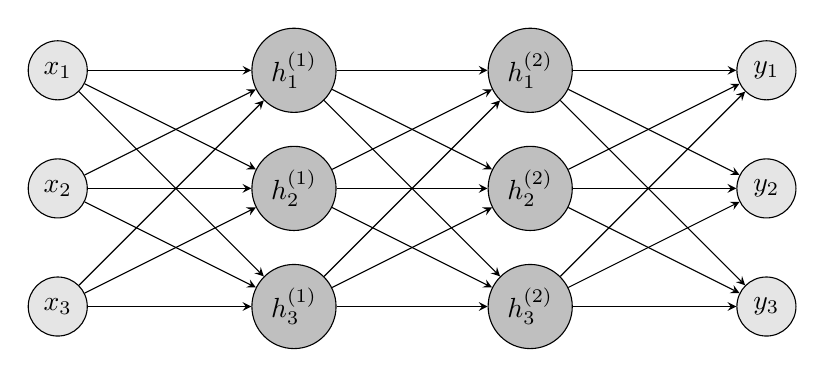
\begin{tikzpicture}[x=1.5cm, y=1.5cm, >=stealth]
  
  % 输入层
  \foreach \m/\l [count=\y] in {1,2,3}
      \node [circle,draw,fill=gray!20,minimum size=0.75cm] (input-\m) at (0,2.5-\y) {$x_\l$};
  
  % 隐藏层
  \foreach \m [count=\y] in {1,2,3}
      \node [circle,draw,fill=gray!50,minimum size=0.75cm] (hidden1-\m) at (2,2.5-\y) {$h_\m^{(1)}$};
  \foreach \m [count=\y] in {1,2,3}
      \node [circle,draw,fill=gray!50,minimum size=0.75cm] (hidden2-\m) at (4,2.5-\y) {$h_\m^{(2)}$};
  
  % 输出层
  \foreach \m [count=\y] in {1,2,3}
      \node [circle,draw,fill=gray!20,minimum size=0.75cm] (output-\m) at (6,2.5-\y) {$y_\m$};
  
  % 连接
  \foreach \m in {1,...,3}
      \foreach \n in {1,...,3}
          \draw [->] (input-\m) -- (hidden1-\n);
  \foreach \m in {1,...,3}
      \foreach \n in {1,...,3}
          \draw [->] (hidden1-\m) -- (hidden2-\n);
  \foreach \m in {1,...,3}
      \foreach \n in {1,...,3}
          \draw [->] (hidden2-\m) -- (output-\n);
  
  \end{tikzpicture}
  \caption{全连接神经网络}
  \label{figure:FCN}
\end{figure}

\xsubsection{卷积神经网络}{Convolutional Neural Networks}
卷积神经网络(Convolutional Neural Networks, CNN)是目前使用范围最广的深度学习模型之一,由其对高维度数据特征提取的能力优异表现而广泛应用于图像处理和计算机视觉任务中。
一般的CNN通常包含卷积层,池化层,全连接层。其常见的模型结构如所示。\cref{figure:CNN}

\begin{figure}[h]
  \centering
\includegraphics[width=0.6\textwidth]{CNN.JPG}
\caption{卷积神经网络结构示意}
\label{figure:CNN}
\end{figure}

卷积层通常利用卷积操作提取图像(或其他输入数据)的空间特征信息。CNN每一层通常具有多个通道(包含多个卷积核),每个卷积和分别与图像进行卷积运算,其的结果将会作为下一层的输入;不同的卷积核可以提取到图像不同类型的空间特征,因此CNN通常相较于FCN有更强大的特征提取能力。
池化层通常用于减小图像尺寸,同时可以保留输入结果中重要的特征信息。常见的池化操作通常有平均值池化(Average Pool)、最大值池化(Max Pool)等。
全连接层则是将CNN的输出结果进行重塑,使得输出维度符合实际需要。通常用于分类或回归预测等任务中。
CNN的运算原理如\cref{equation:CNN}所示。
\begin{equation}
  \label{equation:CNN}
  Y = \sigma\left(\sum_{i=1}^{n} \boldsymbol{W_i} conv(\boldsymbol{X_i}) + \boldsymbol{b}\right)
\end{equation}

其中:
$\mathbf{Y}$ 是输出特征图;
$\sigma(\cdot)$ 是激活函数;
$n$ 是卷积核的数量;
$\mathbf{W}_i$ 是第 $i$ 个卷积核的权重;
$\mathbf{X}_i$ 是与第 $i$ 个卷积核进行卷积的输入特征图;
$\mathbf{b}$ 是偏置项;
$conv(\cdot)$ 表示卷积操作。
自Resnet提出以来\cite{2016Resnet},残差卷积以广泛应用在各种基于卷积神经网络的模型之中其核心思想是通过残差连接来解决神经网络中的梯度消失以及梯度爆炸问题。其模型如\cref{figure:Resnet}
通常这种结构可以使得网络直接学习残差(即残差块的输出减去输入)。本文大量采用了残差卷积块作为模型的基础模块,这种方式可以使整个网络更容易优化和训练,进一步提高网络的性能和泛化能力。
\begin{figure}
  \centering
  \includegraphics[width=0.6\textwidth]{Resnet.png}
  \caption{残差卷积模型}
  \label{figure:Resnet}
\end{figure}



\xsubsection{激活函数}{Activation Functions}

神经网络在各个领域的广泛应用主要得益于其对于非线性映射的强大拟合能力,
这种拟合能力,主要来自于非线性激活函数。
而深度学习模型如CNN,FCN等基础模块的运算通常为大量的线性映射(加法和乘法)。
因此,选择适当的激活函数,对于深度学习模型性能的提升将是显著的。
近年来,各式各样的激活函数不断被学者们提出,本文将重点介绍模型从采用的四种激活函数,如
对于其他未被使用到的激活函数将不做赘述。

\begin{enumerate}

  \item ReLU

ReLU是Hinton于2010年提出的激活函数\cite{2010ReLU},其表达式如\cref{equation:ReLU}所示。
sigmoid函数在函数值趋近于0和1的时候会变得平坦,即此时的梯度几乎为0。而由于神经网络参数更新的方式通过反向传播进行,则此时对于这类输入或输出趋于0或的节点,其权重几乎不会得到更新,此类神经元被称为饱和神经元。
因此,这就会导致神经网络中许多节点的参数不再更新,即梯度消失问题。
ReLU在输入大于0的时候其梯度恒为1,因此可以有效避免梯度消失问题,并且由于其中只存在线性映射,因此能大大提高网络的计算效率,进而加快梯度下降过程中的收敛速度。
此外,该激活函数还被认为具有生物和理性,即与单侧抑制原理相符。

  \begin{equation}
    \label{equation:ReLU}
    \sigma(x) = 
    \left\{
    \begin{aligned}
      0, \quad x <= 0 \\
      x, \quad x > 0
    \end{aligned}
    \right.
    \end{equation}

  \item Sigmoid Linear Unit (SiLU)
  
    SiLU的表达式如\cref{equation:SiLU}所示。
    其相较于ReLU而言,由于其连续可微,故在反向传播的过程中更容易优化。并且SiLU在其定义域内梯度均不为0,这非常有助于在深度神经网络中避免梯度消失的问题。
    同时,由于ReLU函数的特性,网络中输出结果小于0的神经元会被抑制(其梯度为0),故会造成网络稀疏,虽然有助于抑制过拟合,但是也会抑制网络对于数据信息的利用率,进而影响模型的性能。
    并且由于ReLU和Sigmoid函数的输出数据分布的均值均不为零,因此会给给后一层的神经网络引入偏置偏移,进而可能会影响梯度下降的效率。
    而,SiLU的输出范围在$[0, 1]$之间,因此可以为后续的模块保留一定的动态范围,从而有助于更好地处理数据分布的变化。

    \begin{equation}
      \label{equation:SiLU}
      \text{SiLU}(x) = x \cdot \sigma(x)
    \end{equation}
  
    其中,$\sigma(x)$ 是 Sigmoid 函数,定义为:
  \begin{equation}
    \sigma(x) = \frac{1}{1 + e^{-x}}
  \end{equation}
  
  \item Gaussian Error Linear Units function (GeLU)
  
  GeLU是2016年 Hendrycks等人提出的激活函数\cite{2016GeLU}。但直到其在Transformer和Bert模型中得到应用之后,才广泛进入人们的视野。
  该函数的表达式如\cref{equation:GeLU}。
  其中,$\Phi(x)$ 是标准正态分布的累积分布函数(CDF),可以用高斯误差函数(erf)的形式表示。
  GeLU函数通过给输入向量乘以一个权重,该权重是输入变量的非线性映射(即高斯误差函数),其原理与ReLU和Dropout类似。
  不同的是,ReLU会为输入向量乘以固定的权重1(或0),而dropout则会为部分输入乘以0(即抛弃该输入)。
  GeLU所乘的系数,这是与输入变量的自身分布有关。由此,GeLU可以将输入变量$x$平滑地映射到高斯分布的CDF上。
  重要的是,GeLU在最近的深度学习模型中通常表现出优于ReLU或ELU等传统的激活函数。

  \begin{equation}
    \label{equation:GeLU}
    \text{GELU}(x) = x \cdot \Phi(x) 
  \end{equation}
   \begin{equation}
    \label{equation:Gauss}
    \Phi(x) = \frac{1}{2} \left(1 + \text{erf} \left(\frac{x}{\sqrt{2}}\right)\right)
  \end{equation}
  
  特别注意的是,在实现的过程中可以用如\cref{equation:quickGeLU}所示的函数对GeLU作近似估计:
  \begin{equation}
    \label{equation:quickGeLU}
    \text{quickGELU}(x) = \frac{1}{2}x\left(1 + \tanh\left(\sqrt{\frac{2}{\pi}}\left(x + 0.044715x^3\right)\right)\right)
  \end{equation}
  其中,
  \begin{equation}
    tanh(x) = \frac{{e^{x} - e^{-x}}}{{e^{x} + e^{-x}}}
\
  \end{equation}

  \item Softmax

  Softmax函数不同于其他激活函数,其作用是将连续的输出信号映射到离散的空间中,故经常用作分类网络的输出层,其表计算方式如\cref{equation:softmax}所示。
  Softmax计算该层每个神经元的输出对所有神经元输出的和的比值。即此过程将每个神经元的输出映射到了$[0,1]$中,并且输出层
  所有的神经元之和为1。这样做的好处则是输出层的神经元可以表示为一个概率空间,其中每个神经元的输出可以看做是某一个事件发生的概率。
  因此经常作为多分类问题的输出层使用。

\begin{equation}
  \label{equation:softmax}
  \text{softmax}(\mathbf{z})_i = \frac{e^{z_i}}{\sum_{j=1}^{K} e^{z_j}}
\end{equation}

其中,$\mathbf{z} = (z_1, z_2, ..., z_K)$ 是输入向量,$K$ 是类别的数量。softmax 函数将输入向量的每个元素 $z_i$ 转换为相应的概率值,即满足所有概率之和等于1。

\end{enumerate}

\begin{figure}[h]
  \centering
\includegraphics[width=0.7\textwidth]{activation.png}
\caption{激活函数}
\label{figure:activation}
  
\end{figure}

\xsubsection{归一化}{Normalization}
在机器学习(尤其是深度学习)任务中,由于不同通道(特征)数据的量纲往往不同,而这种情况通常会影响最终数据分析的结果。
因此,为了消除这种由于量纲不同而导致模型性能下降的可能性,通常会进行数据标准化(standardization),最常用的方法即数据归一化(Normalization)处理。
简而言之,归一化的目的就是使得预处理的数据被限定在一定的范围内(比如$[0,1]$或者$[-1,1]$),从而消除奇异样本数据导致的不良影响。

本文将重点介绍模型中使用到的以下三种归一化:
\begin{enumerate}
  \item 批归一化(Batch Normalization, BN)

  
  通过计算一个batch中每一个通道内的所有数据的每一个特征的均值和方差,然后利用\cref{equation:norm}
\begin{equation}
  \label{equation:norm}
  res = \frac{x - E\left[ x\right]}{\sqrt{Var\left[ x\right] + \epsilon}} * \gamma + \beta
\end{equation}

其中,$E\left[ x\right], Var\left[ x\right]$分别是上述数据的均值和方差, $\epsilon$为一趋于0的常数,确保分母大于零,
$\gamma, \beta$是可学习的参数,用于对数据进行仿射变换。

该方法可以加快网络的收敛,提高其训练过程的稳定性,还有助于避免产生梯度消失、梯度爆炸的问题。

  \item 组归一化(Group Normalization, GN)
  
  GN将通道划分成若干个组,进而每个组分别进行归一化。其归一化的公式与BN相同。
  
  由于BN通常对batch size 的选择非常敏感,而GN通常选择固定的组数(本文大量使用到GN,其中归一化组数选择为32),
  从而使得归一化的过程不受到batch size的限制,可以有效应用在小批次的样本中。

  \item 层归一化(Layer Normalization, LN)
  LN就是BN在组数为1的特殊情况,即对该次输入所有通道的所有元素进行归一化,该方法同样不依赖于batch size,其更新公式同上。
\end{enumerate}


\xsubsection{优化器}{optimizer}
大多数神经网络的参数更新是通过反向传播算法实现的,其利用损失函数计算输出层的结果与真实的标签数据分布之间的误差,称为网络输出层的损失(loss),然后根据链式法则求出该损失对每一层神经元的参数的损失,然后利用这些损失对网络中每一个参数分别更新。
其中优化器的选择通常决定了如何利用损失函数更新网络参数。

最基础且常见的优化器即为随机梯度下降法(Stochastic Gradient Descent,SGD),在网络模型中的参数初始化之后,该方法首先在训练集中随机选择一个样本,用作本轮计算损失的数据。
然后再利用所选择的损失函数(通常为均方误差损失函数或交叉熵损失函数)计算出输出结果与真实标签分布之间的损失,并利用反向传播算法求出每一步用于更新参数的损失,最后利用\cref{equation:SGD}更新网络参数。

\begin{equation}
  \label{equation:SGD}
  \theta_{t+1} = \theta_{t} - \eta \nabla J(\theta_{t}, x_i, y_i)
\end{equation}
其中,$\theta_{t}$表示第$t$次迭代时模型中的所有参数集,其中包含所有可学习的参数如网络权重等。
$\eta$是学习率(learning rate),用于控制每一步参数更新的步长
$\nabla J(\theta_{t}, x_i, y_i)$则表示损失函数$J$对参数 $\theta_{t}$在样本$i$上的梯度 ;
而$x_i$、$y_i$分别是样本的特征向量(原始数据集中的样本)和样本的标签(label)。
由于随机梯度下降法通常只选择一个样本用来计算梯度,因此训练时间较短,并且训练的方向具有一定的随机性,通常可以跳出局部最优解,从而在更广泛的参数空间中优化网络参数。

但也正是因为其梯度更新方向的随机性,SGD对网络参数更新的频率通常较高,收敛速度可能较慢,并且波动较大,从而导致参数更新不够稳定。

传统的如各种梯度下优化算法通常会将学习率设置为固定值,或硬编码其学习率(如让其成为epoch的函数),这样做就忽略了学习率其他变化的可能性。
因此就产生了自适应学习率优化算法如Adaptive Gradient(AdaGrad)、RMSProp和Adaptive Moment Estimation(Adam)等。

本文在网络模型训练的过程中大量使用了Adam优化算法\cite{2014Adam},这是因为该优化算法通过引入动量项,从而使其具有自适应的学习率(能够根据参数的梯度自动设置学习率,并且该学习率通常有一个固定的范围,这就一定程度上提高了模型参数的稳定性,从而提高了模型收敛的速度,加快了训练过程)。
Adam结合了Adagrad和RMSprop算法的优点,使得其算法更加善于处理稀疏梯度和非平稳目标。
此外也可被用在非凸优化任务中,即适用于大规模的数据集并应用在高维的参数空间中。
Adam优化器在网络模型参数初始化后,还要初始化优化器的超参数,默认$\beta_1 = 0.9$,$\beta_2 = 0.999$控制动量的指数和衰减率;$\epsilon = 10^{-8}$用于防止分母为零,学习率$\eta = 0.001$。
其迭代式如\crefrange{equation:Adamiter:a1}{equation:Adamiter:a5}所示。
\begin{equation}
  \label{equation:Adamiter:a1}
  \centering
  m_t  = \beta_1 m_{t-1} + (1 - \beta_1) g_t
\end{equation}
\begin{equation}
  \label{equation:Adamiter:a2}
  \centering
  v_t  = \beta_2 v_{t-1} + (1 - \beta_2) g_t^2
\end{equation}
\begin{equation}
  \label{equation:Adamiter:a3}
  \centering  
  \hat{m}_t  = \frac{m_t}{1 - \beta_1^t}
\end{equation}
\begin{equation}
  \label{equation:Adamiter:a4}
  \centering
  \hat{v}_t  = \frac{v_t}{1 - \beta_2^t} 
\end{equation}
\begin{equation}
  \label{equation:Adamiter:a5}
  \centering
  \Delta \theta_t  = -\frac{\eta}{\sqrt{\hat{v}_t} + \epsilon} \hat{m}_t 
\end{equation}
\begin{equation}
  \label{equation:Adamiter:a6}
  \theta_{t+1} = \theta_t + \Delta \theta_t 
\end{equation}
其中,$m_t, v_t$分别表示一阶和二阶动量,$\hat{m}_t, \hat{v}_t$分别表示对一阶以及二阶动量校正偏差后的值的估计。
$\Delta\theta_t$ 表示每部参数更新的量,$\theta_t$表示第$t$步中网络参数值。


\xsubsection{注意力机制}{attention}
注意力机制(Attention)是由 Bahdanau等人于2014年提出的\cite{2014Neural},最初应用于自然语言处理领域,此后由于其性能优秀而广泛应用在各个领域。
attention机制让神经网络能够关注输入数据的某些相关的信息,而减少对无用信息的关注。这种思想源于人们的视觉系统,即人们在看到一张图片或视频时通常会关注其中感兴趣的部分。

attention通常包含三个重要的部分,即:
\begin{enumerate}
  \item 查询矩阵(query, Q): 其中的值代表模型应该更加关注输入数据中的某些部分,即Q作为输入向量的某种表示,可以反映模型更加需要关注的内容。
  \item 键(key, K):表示输入向量的特征。
  \item 值(values, V):是K对应输入向量的另一维度的特征,用于和QK所获得的的相似度进行加权和。
\end{enumerate}

其基本原理为:首先计算出Q和K的相似度,然后利用Softmax进行归一化算出每个元素所对应各权重,最后利用上一步计算的结果与V中的元素做加权和,以输出最终的结果。
其中,由于相似度计算方式的不同以及Q、K、V选择方式的不同,就产生了attention的各种应用以及变体,包括自注意力机制(Self-attention),交叉注意力机制(Cross-attention)等。


\xsection{生成式模型}{Generative Models}
EIT图像重建算法的任务目标即是在给定边界条件下生成出符合原始电导率分布的图像。
通常基于深度学习模型设计的EIT图像重建算法利用电压-电导率分布数据构件数据集,学习出电压到电导率分布的非线性映射以实现对EIT待测场中的目标信息进行成像。
此类深度学习模型的目标是估计$p(C \mid v)$(在已有的观测数据分布上估计目标变量的概率分布),其中$C$是电导率分布的真实概率分布,$v$是测量电压构成的向量组。
而实际情况下该很难拟合出上述复杂的概率分布模型,故深度学习模型通常有两类不同的做法,即判别式模型和生成式模型。

判别式模型如卷积神经网络等通常通以$P(C \mid V=v)$为目标,即拟合$f(v) = p(c \mid v)$这一非线性映射。
不同于判别式模型,生成式模型则是先估计出$p(v \mid c)$ 再通过贝叶斯公式(\cref{equation:bysf})计算出$p(c \mid v)$。
\begin{equation}
  \centering
  \label{equation:bysf}
  p(c \mid v) = \frac{p(c, v)}{p(v)} = \frac{p(v \mid c)p(c)}{p(v)} 
\end{equation}

故生成式模型的本质是建立一个映射$X=g(Z)$,从隐变量的分布(latent variable)$Z$生成数据的真实分布。通常假设隐变量的分布为高斯分布(Gaussian Distribution)。
生成式模型的学习目标即通过一组数据($\mbs{X} = \{X_1, X_2, ..., X_i\}, i = 1, 2, ..., n$)学习其真实分布$p(X)$。即假设该数据集是从一个概率分布$p(x)$中采样的结果,生成式模型希望根据该采样结果(即数据集)恢复出这个概率分布。此后通过采样即可生成符合此分布的数据。
而由恢复该分布较为困难,因此根据贝叶斯公式,在此过程中引入隐变量$Z$,利用隐变量$Z$与原始数据的关系计算出原始数据的概率分布$p(x)$,如\cref{equation:GenerativeModel}(离散情况),\cref{equation:GenerativeModelcon}(连续情况)。

\begin{equation}
  \centering
  \label{equation:GenerativeModel}
  P(x) = \sum_{Z}^{}p(x\mid Z)p(Z)
\end{equation}

\begin{equation}
  \centering
  \label{equation:GenerativeModelcon}
  p(x) = \int_{z \in Z}^{} p(x|z)p(z)\diff z
\end{equation}

变分自编码器(Variational Auto Encoder, VAE)就是生成式模型的一种,如\cref{figure:VAE}所示。其编码器将原始的数据分布$\mathbb{R}^n$映射到隐变量空间$\mathbb{R}^d$中,其隐变量空间为一组高斯分布的均值和方差。
\begin{figure}[h]
  \centering
  \includegraphics[width=.7\textwidth]{VAE.png}
  \caption{VAE架构}
  \label{figure:VAE}
  \end{figure}

即该编码器需要通过已知的观测样本$\mbs{X}$,计算出$p(z|x)$,如式\cref{equation:bysVAE}。

\begin{equation}
  \centering
  \label{equation:bysVAE}
  p(z \mid x) = \frac{p(x \mid z)p(z)}{p(x)} 
\end{equation}

然而,由于无法事先确定数据集采样的源分布$p(x)$,因此VAE通过利用一个可控制的分布$q(z|x)$来近似估计$p(z|x)$。
而由于K-L散度(Kullback-Leibler divergence,)可以很好地度量两个概率分布$P$和$q$之间的差异(该度量为非对称性的,如\cref{equation:KLdivergence}),

\begin{equation}
  \centering
  \label{equation:KLdivergence}
  D_{\text{KL}}(P \| Q) = \int_{x} P(x) \log \left( \frac{P(x)}{Q(x)} \right)
\end{equation}
故VAE的本质即最小化$p(z|x)$和$q(z|x)$的K-L散度(如\cref{equation:VAEKL})。
\begin{equation}
  \centering
  \label{equation:VAEKL}
  \min D_{\text{KL}}(q(z|x)\|p(z|x)) = \int_{x}q(z|x)\log \frac{q(z|x)}{p(z|x)}\diff Z
\end{equation}
上式经过计算可等价为\cref{equation:KLeq},
\begin{equation}
  \centering
  \max  \mathbb{E}_{z\sim q(z|x)} \log p(x|z) - D_{\text{KL}}(q(z|x)\|p(z))
  \label{equation:KLeq}
\end{equation}
即,最大化在$z$上采样的结果经过VAE后输出的重构结果为$x$的概率(等价于最小化网络输出结果与真实数据之间的均方误差),且让$q(z|x)$和$p(z)$尽可能相似。


除了VAE之外,Jonathan Ho等人提出的去噪的扩散概率模型\cite{DDPM}(Denoising Diffusion Probabilistic Models, DDPM)以及后续的各种变体如条件扩散模型\cite{CondDDPM}(Conditional Denoising Diffusion Probabilistic Models),稳定扩散\cite{StableDiffusion}(Stable Diffusion)等已在图像生成领域取得了显著的成绩。
扩散模型的思想源于非平衡统计物理,其通过迭代完成正向的扩散过程从而系统、缓慢地破坏数据的结构。此后利用深度学习模型学习逆扩散的过程,从而恢复数据中的结构。由此产生了一个高度灵活且易于处理的数据生成模型。
其中,扩散的迭代次数通常可设定为千次左右。

该模型共包含两个主要部分,即正向扩散部分和逆向数据恢复部分。均可看作是一个参数化的马尔科夫链(Markov Chain)。
该模型同样是一个隐变量模型,即$p_\theta(x_o) \coloneqq \int p_\theta(x_{0:T})\diff x_{1:T}$,其中$x_1,...x_T$为隐变量,其大小和输入的$x_0$相同。

正向或(扩散)过程(froward process 或 diffusion process)如\cref{figure:Diffusionforward}所示。

\begin{figure}[h]
  \includegraphics[width=.7\textwidth]{diffusionforward.png}
  \caption{DDPM加噪过程}
  \label{figure:Diffusionforward}
\end{figure}

该过程通过向原始的数据中不断加入已知的高斯噪声,随着噪声的不断增加该数据将趋近于一个高斯分布。
其中,$x_0$是原始的数据分布,$x_1, x_2,..,x_t$,$t=1:T$是第$t$步加噪声后的结果。
由于马尔科夫链中第$t$步的$x_t$只与$t_1$时刻的$x_{t-1}$有关,故可得近似后验概率$q(x{1:T}|x_0)$为:

\begin{equation}
  \centering
  q(x_{1:T}|x_0) = \prod_{t=1}{T} q(x_t|x_{t-1}) \qquad
  q(x_t|x_{t-1}) = \mathcal{N}(x_t; \sqrt{1-\beta_t}x_{t-1}, \beta_t\mbs{I})
\end{equation}
其中,$t$为时间轴,通常定义为$0-1000$(线性,也可以为cosine等),$\beta_t$是方差序列(variance schedue)用来控制噪声与信号混合的比例,
满足$\beta_1 < \beta_2 <...<\beta_T$。
经推导\cite{DDPM}可得出$t$t时刻的隐变量$x_t$可由原始数据分布$x_0$得到:
\begin{equation}
  \centering
  q(x_t|x_0) = \mathcal{N}(x_t; \sqrt{\bar{\alpha_t}x_0}, (1-\bar{\alpha}\mbs{I}))
\end{equation}

其中,逆向过程(resverse process)是从一个高斯分布中不断去噪声,从而恢复出原始的数据分布的过程,如\cref{figure:Diffusionreverse}所示。

\begin{figure}[h]
  \centering
  \includegraphics[width=.7\textwidth]{diffusionreverse.jpg}
  \caption{DDPM去噪过程}
  \label{figure:Diffusionreverse}
\end{figure}

该过程定义为$p_\theta(x_{0:T})$,则只要得到$q(x_{t-1}|x_t)$,就可以从一个高斯噪声中还原出原本的数据点$x_0$。
该模型利用$p_\theta(x_{t-1}|x_{t})$来近似该分布。
\begin{equation}
  \centering
  p_\theta(x_{T}) = \prod_{t=1}{T} q(x_{t-1}|x_{t}) \qquad
  p_\theta(x_{t-1}|x_{t}) = \mathcal{N}(x_{t-1}; \mu_\theta(x_t, t), \Sigma_\theta(x_t, t))
\end{equation}

在上式中,均值
\begin{equation}
  \mu_\theta = \frac{1}{\sqrt{\alpha_t}}(x_t - \frac{\beta_t}{\sqrt{1-\hat{\alpha_t}}}\epsilon_\theta(x_t, t))  
\end{equation}
故只需要利用神经网络拟合出从$t$时刻到$t-1$时刻所需要添加的噪声$\epsilon_\theta(x_t, t)$网络即可推断出原始的数据点。

去噪声网络通常利用U-net实现,其通过最小化每一步骤中真实加入的噪声和该网络生成的噪声的均方误差从而训练整个网络使其收敛。
此后,该模型正向推理的过程从一个高斯噪声开始,经过$T:1$时刻通过训练好的去噪网络分别计算出每个时刻需要去掉的噪声,从而获得生成的最终结果。


\xsubsection{小结}{Summary}
本章首先介绍了EIT技术的基本原理、传统EIT图像重建算法的实现过程以及其弊端。
随后介绍了常见的深度学习模型以及本文所使用到的深度学习相关技术。
最后介绍了实现本文所提出的EIT图像重建算法所用到的生成式模型,主要包括VAE的架构和扩散模型的基本原理。
为后续实现图像重建算法提供了理论基础。

% !TeX root = ../main.tex

\xchapter{生成式EIT图像重建算法的设计与实现}{Design and Implementation of Generative EIT Reconstruction Algorithm}
传统的EIT图像重建算法通常利用迭代的思想多次求解EIT正问题、逆问题,以不断最小化每一步求解的电压分布和真实电压分布之间的误差。
这种做法通常消耗时间长,成像分辨率低。由于EIT正问题仿真模型完备,且相对精确,而常见的深度学习模型则需要大量的训练数据,
因此基于深度学习的EIT图像重建模型大大提高了EIT图像重建算法的图像重建分辨率。
并且由于训练好的深度学习模型正向推理的过程通常耗时较少,因而能显著提高图像重建算法的时间效率。
这也为EIT技术实现床旁实时监测、院前疾病检测提供了技术保障。

目前主流的利用深度学习技术实现的EIT图像重建算法通常以卷积神经网络的各种变体为模型基础,
通过添加具有不同功能的模块来优化网络性能。
此类方法通常使用判别式模型来实现。

扩散概率模型,作为生成式模型的一种,近年来在图像生成领域已经取得了显著的成果。而EIT图像重建问题本质上是建立从电压分布到电导率分布的非线性映射,
即可以看作是生成目标为电导率分布,且指导模型生成电导率分布的条件为电压分布的带条件的扩散概率模型。
利用扩散模型实现的EIT图像重建算法由于其模型固有的优势而能更好地拟合电导率的原始概率分布。并且通过对扩散过程的改进,可
以有效减少在推理过程中的采样次数,极大程度地缩短了模型正向计算的过程,进而提高了EIT图像重建效率。

本章将提出一个生成式EIT图像重建算法,并重点介绍其设计理念与实现过程。包括算法的流程、EIT图像重建模型总体的结构、模型各部分的结构和作用、
模型训练集的设计和仿真、训练过程、训练结果以及对模型性能的评估和优化。


\xsection{生成式EIT图像重建算法设计}{Design of Generative EIT Reconstruction Algorithm}


EIT图像重建算法就是要利用场域边界电压-电流数据重构出其内部电导率分布。
但是,电流的激励方式、电压信号的维度等都会影响到EIT图像重建算法的设计,并且同一类型的数据也包含多种表示方式(如电压可表示为矩阵形式和向量形式)。
因此本节首先定性和定量地描述EIT图像重建问题,随后将提出一个生成式EIT图像重建算法。

\xsubsection{EIT图像重建问题分析}{Analysis of EIT Image Reconstruction Problem}

设如\cref{figure:xyz}所示的待测场$\Omega$所包含的剖分单元个数为$d_e$,边界为$\partial \Omega$。其边界的电极个数为$d_v$。
EIT采集系统的激励模式为邻近激励,单次测量所有激励模式所构成的集合为$S_{stim}$,单次测量电流激励的次数为$n_m$;测量电压的模式为邻近差分,单次激励测量电压的维度为$d_{vm}$。
则单次测量的电压向量维度为$d_m = d_{vm} * n_m$。(关于EIT的有限元模型和测量模式详见\cref{PrincipleEIT})。
利用上述测量模式,可获得EIT测量电压分布。EIT的测量电压共包括两个部分,分别为背景帧的边界电压以及含扰动目标的边界电压。
其中,背景帧的边界电压分布可分别表为矩阵形式$v_{0mtx} = \{v_{ij}\}, i \in S_{stim}, j =1,2,...d_{vm}$,向量形式$v_{0vector}$。
含扰动目标的边界电压分步的两种形式分别为$v_{mtx} = \{v_{ij}\}, i \in S_{stim}, j =1,2,...d_{vm}$。向量形式$v_{vector}$,
其中$v_{ij}$表示以$i$为激励方式的第$j$次测量的结果,向量的维度为$d_m$。

\begin{figure}[h]
    \centering
    \includegraphics[width=.5\textwidth]{eeeee.png}
    \caption{待测场图示}
    \label{figure:xyz}
  \end{figure}


则EIT图像重建算法的目标为通过测量含扰动目标的边界电压以及背景帧的边界电压的差$\Delta v_{vectore} = v_{vector} - v_{0vector}$重建出其场域内部的的电导率分布变化向量 $\sigma$,其维度为 $1 \times d_e$。
EIT重建的图像分辨率为$res_{row} \times res_{column}$。

如无特殊说明,本文所采用的参数均为\cref{table:param_stm}中的默认值。
\begin{table}[h]
    \centering
    
    \caption{参数设置}
    \begin{tblr}{
        colspec = {X[c] X[c] X[c] X[c]},
    }
    \toprule
    参数 & 值(域) & 参数 & 值(域) \\
    \midrule
    $\Omega$ & 圆形场域 $ x \in [-1, 1], y \in[-1, 1]$ & $S_{stim}$ & [i, i+1], i=(0:15)\%15 \\
    $d_e$ & 1024 & $n_m$ & 16 \\
    $d_v$ & 16 & $d_{vm} $ & 16 \\
    $d_m$ & 256 & $\sigma_i$ & $[1, d_e]$ \\
    $res_{row}$ & 16 & $res_{column}$ & 16 \\

    \bottomrule
    \end{tblr}
    \label{table:param_stm}
\end{table}

\xsubsection{生成式EIT图像重建算法总述}{Overall of of Generative EIT Reconstruction Algorithm for Fast Detection of Stroke}

根据上一节所提出的EIT图像重建问题,本节提出了一个用于脑卒中快速鉴别的生成式EIT图像重建算法,
由于其应用EC-Diffusion模型实现而命名为EC-Diffusion算法如\cref{algorithm:GeneAlgorithm}和\cref{figure:AlgorithmEIT}。
\begin{figure}[h]
    \centering
    \includegraphics[width=.8\textwidth]{AlgorithmEIT.png}
    \caption{生成式EIT图像重建算法}
    \label{figure:AlgorithmEIT}
\end{figure}

\begin{algorithm}[H]
    
    \caption{生成式EIT图像重建算法}
    \begin{algorithmic}[1]
        \State 测量未知场域不含扰动目标的边界电压$v_{0vector}$
        \State 测量含有扰动目标时该场域的边界电压$v_{vector}$
        \State 计算边界电压差向量$\Delta v_{vector} = v_{vector - v_{0vector}}$
        \State 获得训练好的EC-Diffusion 模型 $\text{EC-Diffusion}(\cdot)$
        \State \textbf{Input:} $\Delta v_{vecotr}$
        \State \textbf{Output:} $ \sigma  = \text{EC-Diffusion}(\Delta v_{vecotr})$
    \end{algorithmic}
    \label{algorithm:GeneAlgorithm}
\end{algorithm}

在该算法中,“获得训练好的EC-Diffusion模型”共需要三个阶段实现,分别是:

1)设计并实现用于EIT图像重建任务的模型。该阶段使用改进的扩散模型作为EIT图像重建算法的核心模块,因此还需要对原始的
电压数据进行处理,故该阶段采用了一个编码器-解码器结构分别对重建前的电压数据进行编码(预处理)以及对重建后的电导率分布进行解码(后处理)。
由于该模型利用Diffusion Model通过编码后的电压分布重建出编码后的电导率分布,故将其命名为EC-Diffusion(Encoded Diffusion)。

2)模型训练。这一阶段会使用仿真软件仿真出用于训练模型所需要的EIT数据,并利用这些数据训练模型至收敛。

3)模型评估。将用于测试网络性能的数据输入至训练好的模型,并根据其重建出的图像以及其他参数评估模型性能并优化模型。

上述阶段利用EIT数据使EC-Diffusion模型学习到最优的参数,以尽可能地拟合EIT电压-电导率分布。
当以上阶段完成后,便可利用\cref{algorithm:GeneAlgorithm}解决EIT图像重建问题。即,
将EIT边界差分电压数据输入至训练好的模型中,经过模型正向推理即可得到其内部电导率分布的图像。


\xsection{EC-Diffusion模型的设计与实现}{Design and Implementation of the EC-Diffusion Model}

EC-Diffusion模型是实现本文所提出的EIT图像重建算法的核心部分,故本节将首先介绍该模型的总体架构,
随后将分别对该模型中电压编码块、图像重建块和图像后处理块的设计与实现展开详细的介绍。

\xsubsection{模型的总体架构}{Overall of the Model Architecture}
\label{section:Model}

针对EIT图像重建问题中的非线性映射,
本文提出了一个利用编码器-解码器以及一个基于改进扩散模型的深度生成式EIT图像重建模型:EC-Diffusion,如\cref{figure:EITREmodel}所示,

\begin{figure}[h]
    \centering
    \includegraphics[width=.9\textwidth]{EITREmodel.png}
    \caption{EC-Diffusion 模型}
    \label{figure:EITREmodel}
\end{figure}
该模型共包括三个模块,分别是:

1)电压编码块(Voltage Encoding Block):由一个电压编码器(Voltage Encoder, VEncoder)构成。用于对电压数据进行编码,以输出适应图像重建块的输入维度。

2)图像重建块(即基于扩散模型的图像重建快,Diffusion-Based Reconsturction)。该部分利用改进的扩散概率模型拟合EIT图像重建问题中的非线性映射,输出编码后的电导率分布。该模块是本算法的核心部分。

3)图像后处理块(即电导率解码块,Conductivity Decoding Block)。由一个电导率解码器(Conductivity Decoder, CDecoder)构成。用于解码图像重建块的生成结果,将生成结果映射到用于引导EIT图像的电导率分布。

则该模型将首先利用VEncoder对EIT电压数据进行编码,随后将编码后的电压输入到图像重建块中,获得图像重建结果。需要注意的是,
该图像重建块重建出的结果同样为编码后的图像,因此还需要利用一个CDecoder对编码后的图像进行解码,解码后的结果即为该模型重建后的EIT图像。
以下将分别介绍上述三个模块的设计与实现。



\xsubsection{电压编码块}{Voltage Encoding Block}


VEncoder的编码目标是使得编码后的结果尽可能表达出更强有关于该电压数据所对应的电导率分布的特征,
而CNN对于高维数据的空间特征提取能力具有显著的优势,同时,CNN也相较于MLP而言具有更少的可学习参数。因此,此节以CNN为主体,利用径向基函数神经网络(Radial Basis Function Neural Network, RBFNN)
实现了一个RBF-CNN结构的编码器,其结构如\cref{figure:RBFCNN}所示。
\begin{figure}[h]
    \centering
    \includegraphics[width=.9\textwidth]{RBFCNN.png}
    \caption{VEncoder编码器架构}
    \label{figure:RBFCNN}
\end{figure}

其中,Conv3$\times$3为卷积层,卷积核大小为3$\times$3;Max pool 为最大池化层;Average pool为平均值池化层。

RBF则为RBFNN层,
与 MLP 不同,RBFNN 使用欧几里德距离和高斯激活函数,这使得神经元对局部信息更加敏感。 
RBF 网络具有与 MLP 类似的输入层和输出层。
不同的是,隐藏层中的每个神经元都有一个原型向量和一个由 $\mu$ 和 $sigma$ 表示的带宽分别计算输入向量与其原型向量之间的相似度,如\cref{equation:RBFNN}所示。
\begin{equation}
    \label{equation:RBFNN}
    y(x) = f(z(x)) = \sum_{i=1}^{m} v_i \phi_i(z(x)) + b
\end{equation}
其中:
\begin{equation}
    \phi_i(z(x)) = \exp\left(-\frac{|x - \mu_i|^2}{2\sigma_i^2}\right)
\end{equation}

$y(x)$ 是 RBFNN 的输出;
$f(\cdot)$ 是输出层的激活函数;$z(x)$ 是隐含层的输出;
$\phi_i(z(x))$ 是隐含层神经元 $i$ 的激活函数;
$v_i$ 是连接隐含层和输出层的权重;
$b$ 是偏置项;
$m$ 是隐含层神经元的数量。

SelfAttention层为自注意力机制层,由一个LayerNorm层 和一个SelfAttention模块和组合而成。
如\cref{figure:Selfatt}所示。
\begin{figure}[h]
    \centering
    \includegraphics[width=.9\textwidth]{Selfatt.png}
    \caption{SelfAttention 层}
    \label{figure:Selfatt}
\end{figure}

注意力机制(Attention)是由 Bahdanau等人于2014年提出的\cite{2014Neural},最初应用于自然语言处理领域,此后由于其性能优异而广泛应用在各个领域。
注意力机制让神经网络能够关注输入数据的某些相关的信息,而减少对无用信息的关注。这种思想源于人们的视觉系统,即人们在看到一张图片或视频时通常会关注其中感兴趣的部分。

Attention通常包含三个重要的部分,即:

  1) 查询矩阵(query, Q): 其中的值代表模型应该更加关注输入数据中的某些部分,即Q作为输入向量的某种表示,可以反映模型更加需要关注的内容。
  
  2) 键(key, K):表示输入向量的特征。

  3) 值(values, V):是K对应输入向量的另一维度的特征,用于和QK所获得的的相似度进行加权和。


其基本原理为:首先计算出Q和K的相似度,然后利用Softmax进行归一化算出每个元素所对应的权重,最后利用上一步计算的结果与V中的元素做加权和,以输出最终的结果。
其中,由于相似度计算方式的不同以及Q、K、V选择方式的不同,就产生了Attention的各种应用以及变体,包括自注意力机制(Self-Attention),交叉注意力机制(Cross-Attention)等。

SelfAttention层是注意力机制的一种应用,其具体的计算过程如\cref{algorithm:Self_attention}。该机制允许模型在处理电导率分布时专注于数据的某些部分(如扰动目标的部分),而忽略其他部分(即背景帧)。
该模块可以使得电导率分布在不同的位置之间保持联系,以实现对扰动部分更好地成像。

\begin{algorithm}

\caption{Self Attention Layer}
\begin{algorithmic}[1]
    \State \textbf{Input:} 输入向量 $\boldsymbol{X}$代表网络中的隐变量。
    \State 初始化权重矩阵:$W_Q$, $W_K$, $W_V$
    \State 计算Q、K、V:$Q = XW_Q, \quad K = XW_K, \quad V = XW_V$
    \State 计算Attention:$A = \text{softmax}\left(\frac{QK^T}{\sqrt{d_k}}\right) \quad $ $d_k$ 为Q和K的维度 
    \State 计算加权后的结果:$Z = AV$
    \State 对Z进行线性变换,获得Self-Attention最终的输出 :$\text{Self-Attention}(X) = ZW_O$
    \State \textbf{Output:} $\text{Self-Attention}(X)$
\end{algorithmic}
\label{algorithm:Self_attention}
\end{algorithm}

具体而言, 由于EIT图像重建任务中,其电导率分布按照扰动目标的存在与否通常可被分为两个部分:背景帧溶液和扰动目标部分。
其中,背景帧部分通常模拟电导率分布相对固定的电解质溶液,用于代表正常脑组织的区域。这部分通常对于EIT成像结果影响较小(即应该降低该部分对于EIT图像重建结果的影响),因此需要降低模型对于该部分的关注度。
而扰动目标区域则用于模拟特定的病灶区域(由于这些区域的含水量与背景帧不同而导致的电导率变化)。这部分通常对于EIT成像结果影响显著(即扩大该部分数据对于EIT重建结果的影响)。
而Self Attention机制通过计算一组数据内部的相关性并对每个元素重新赋上加权和,可以有效的关注其输入数据的特定部分。因此在此处引入Self Attention层将一定程度上提高扰动目标区域对电压分布或电导率分布中相关部分的关注程度,
进而可以有效地提高网络对EIT非线性映射的拟合能力。

LN层为层归一化层(Layer Normalization, LN),用于对上一层的输出归一化。
LN对该次输入所有通道的所有元素进行归一化(计算所有输入的均值和方差),然后利用\cref{equation:norm}对其进行更新。
\begin{equation}
  \label{equation:norm}
  res = \frac{x - E\left[ x\right]}{\sqrt{Var\left[ x\right] + \epsilon}} * \gamma + \beta
\end{equation}

其中,$E\left[ x\right], Var\left[ x\right]$分别是上述数据的均值和方差, $\epsilon$为一趋于0的常数,确保分母大于零,
$\gamma, \beta$是可学习的参数,用于对数据进行仿射变换。
由于该层在运算的过程中不受到batch size的限制,故可以有效应用在小批次的样本中。此外,该方法可看作是组归一化中组数为1的特殊情况。


此外,该编码器中的GELU层为激活函数层,利用GELU作为激活函数。在对GELU实现时,本文采用如\cref{equation:quickGeLU}所示的函数对GeLU作近似估计:
  \begin{equation}
    \label{equation:quickGeLU}
    \text{quickGELU}(x) = \frac{1}{2}x\left(1 + \tanh\left(\sqrt{\frac{2}{\pi}}\left(x + 0.044715x^3\right)\right)\right)
  \end{equation}
  其中,
  \begin{equation}
    tanh(x) = \frac{{e^{x} - e^{-x}}}{{e^{x} + e^{-x}}}
\
  \end{equation}
由于GELU本身运算复杂,因此该做法可有效提高网络的运算效率。


\xsubsection{图像重建块}{Image Reconstruction Block}

图像重建块的目标即为利用编码后的电压数据重建出编码后的电导率分布图像,如\cref{figure:ReconsBlock}所示。
\begin{figure}[h]
    \centering
    \includegraphics[width=.7\textwidth]{ReconsBlock.jpg}
    \caption{图像重建块}
    \label{figure:ReconsBlock}
\end{figure}

由于扩散模型在图像重建、图像生成、图像超分辨率等领域均取得了广泛的应用和显著的成绩,故此模块考虑利用扩散模型作为主体来拟合EIT图像重建过程。
原始的扩散模型通过对一组数据分布进行拟合,从而输出同分布的数据。而EIT图像重建任务中,电导率分布通常由电压分布引导而来,故该模型还需要通过电压数据引导,
从而生成特定电压分布下对应的电导率分布结果。以下将具体介绍该模型的实现方式。

对于EIT图像重建过程,本文建立了如下的扩散模型:

假设假设原始的电导率分布为$\mbs{x}_0$,原始电导率分布分布模型可以表述为
$p_\theta(\mbs{x}_0) \coloneqq \int p_\theta(\mbs{x}_{0:T})\diff x_{1:T}$。则扩散过程(Diffusion Process)和逆扩散过程(Reverse Process)可描述为如下方式:

\subsubsection{扩散过程}

扩散过程,也被称为正向过程(Forward Process),如\cref{figure:dp}。通过向原始的电导率分布中不断加入已知的高斯噪声,
随着噪声的不断增加该数据分布将趋近于一个高斯分布。

\begin{figure}[h]
    \centering
    \includegraphics[width=.95\textwidth]{DP.jpg}
    \caption{正向过程}
    \label{figure:dp}
\end{figure}

该过程通过一个用一个控制噪声与信号混合比例的方差序列(Variance Schedule)$\beta_1, ...\beta_T$,向电导率分布中逐渐添加高斯噪声。满足$\beta_1 < \beta_2 <...<\beta_T$。

由于马尔科夫链中第$t$步的$\mbs{x}_{t}$只与$t-1$时刻的$\mbs{x}_{t-1}$有关,故可得给定原始电导率分布$\mbs{x}_0$时近似后验$q(\mbs{x}_{1:T}|\mbs{x}_0)$为:
\begin{equation}
    \centering
    q(\mbs{x}_{1:T}|\mbs{x}_0) = \prod_{t=1}^{T} q(\mbs{x}_{t}|\mbs{x_{t-1}}) \qquad
    q(\mbs{x}_{t}|\mbs{x}_{t-1}) = \mathcal{N}(\mbs{x}_{t}; \sqrt{1-\beta_t}\mbs{x}_{t-1}, \beta_t\mbs{I})
    \label{equation:ddpm_f}
  \end{equation}

其中,$t$为时间轴(线性),定义为$[0,1,2,...,1000]$。
$\mbs{x}_1, \mbs{x}_2,..,\mbs{x}_{t}$,$t=1:T$是第$t$步加噪声后的结果。如此可保证$\mbs{x}_{t}$在$t$时刻有较小的信噪比,
即近似后验$q(\mbs{x}_{T}|\mbs{x}_0)$接近于一个同维度的标准正态分布。

经推导可得出$t$时刻的隐变量$\mbs{x}_{t}$可由原始数据分布$\mbs{x}_0$得到:
\begin{equation}
  \centering
  q(x_t|x_0) = \mathcal{N}(x_t; \sqrt{\bar{\alpha_t}x_0}, (1-\bar{\alpha}\mbs{I}))
\end{equation}


\subsubsection{逆扩散过程}

逆扩散过程(Reverse Process)是一个可学习的马尔科夫链(Markov Chain)。如\cref{figure:revs}所示。

\begin{figure}[h]
    \centering
    \includegraphics[width=.95\textwidth]{revs.jpg}
    \caption{逆扩散过程}
    \label{figure:revs}
\end{figure}

该过程将从$T$时刻的隐变量$\mbs{x}_{t}$,
即一个高斯分布$p_\theta(\mbs{x_{0:T}}) = \mathcal{N}(\mbs{x}_{t}; \mbs{0},\mbs{I})$开始,通过不断去噪声,从而恢复出原始的电导率分布。
该过程定义为$p_\theta(x_{0:T})$,如\cref{equation:ddpm_r},则只要得到$q(x_{t-1}|x_t)$,就可以从一个高斯噪声中还原出原本的数据点$x_0$的分布。
\begin{equation}
    \centering
    p_\theta(\mbs{x}_{T}) = \prod_{t=1}{T} q(\mbs{x}_{t-1}|\mbs{x}_{t}) \qquad
    p_\theta(\mbs{x}_{t-1}|\mbs{x}_{t}) = \mathcal{N}(\mbs{x}_{t-1}; \mu_\theta(\mbs{x}_{t}, t, \mbs{v}), \Sigma_\theta(\mbs{x}_{t}, t, \mbs{v}))
    \label{equation:ddpm_r}
\end{equation}

其中,$\mu_\theta(\mbs{x}_{t}, t, \mbs{v})$和$\Sigma_\theta(\mbs{x}_{t}, t, \mbs{v})$分别为$p_\theta(\mbs{x}_{t-1}|\mbs{x}_{t})$
的均值和方差。

由此可以看出,只要获得$\mu_\theta(\mbs{x}_{t}, t, \mbs{v})$和$\Sigma_\theta(\mbs{x}_{t}, t, \mbs{v})$,就可以根据上述马尔科夫链求解出
原始的电导率分布。

在上式中,经推导可得,均值
\begin{equation}
  \mu_\theta = \frac{1}{\sqrt{\alpha_t}}(\mbs{x}_{t} - \frac{\beta_t}{\sqrt{1-\hat{\alpha_t}}}\epsilon_\theta(\mbs{x}_{t}, t, v))  
\end{equation}
而方差则可由方差序列得到。
则进一步可以看出,只需要得到从$t$时刻到$t-1$时刻需要去掉的噪声$\epsilon_\theta(\mbs{x}_{t}, t, v)$,
即可递推地重建出$t=0$时刻的原始电导率分布$\mbs{x}_0$。故只需要利用神经网络拟合出所需要添加噪声的网络即可推理出原始的数据分布。

\subsubsection{图像重建块的实现}

根据上述设计,本文首先设计并实现了一个用生成噪声的网络NoiseG,以对隐变量去噪。
随后按照如\cref{figure:ReconsModel}实现了上述模型。


\begin{figure}[h]
    \centering
    \includegraphics[width=1\textwidth]{ReconsModel.PNG}
    \caption{图像重建块模型结构}
    \label{figure:ReconsModel}
\end{figure}

在推理阶段时,首先随机生成一个大小为$32\times 32$的高斯噪声(与电导率分布编码后的大小相同)作为$t$时刻的隐变量$\mbs{x}_{t}$,
然后通过向训练好的NoiseG中输入该时刻的隐变量$\mbs{x}_t$、当前时刻$t$以及经过上一节中电压编码器VEncoder编码后的电压向量$\mbs{v}$,
输出上一时刻的隐变量$\mbs{x}_{t-1}$,经过不断迭代最终输出该电压分布作为边界条件所对应的电导率分布(编码后)。

NoiseG网络以U-net作为基本结构,如\cref{figure:Unet}所示。U-net是由Olaf Ronneberger等人于2015年提出的基于CNN的深度学习模型\cite{2015U},该网络在医学图像分割领域取得了优异的表现,
此后该网络被广泛应用在各个领域,包括DDPM的去噪网络中\cite{DDPM},该网络是一个典型的编码器-解码器结构,由一个编码器和一个解码器组成,
其中,编码器将输入信号映射到隐空间中,解码器对隐空间中的数据进行解码,进而获得想要的结果。

\begin{figure}[h]
    \centering
    \includegraphics[width=1\textwidth]{Unet.png}
    \caption{NoiseG网络架构}
    \label{figure:Unet}
\end{figure}

该网络以残差卷积块(ResidualBlock)为主要结构(即图中蓝色箭头所表示的运算),
该模块不仅包上一层的输出$x$,还包含了时刻信息$t$,如\cref{table:Unet}所示。

\begin{table}[h]
    \centering
    \caption{Unet中ResidualBlock的结构}
    \label{table:Unet}
    \begin{tblr}{
        colspec = {X[c, 0.5] X[c] X[c] X[c, 2]},
        }
        \toprule
        层数 & 输入 & 网络类型  & 输出\\
        \midrule
        1 & $input$ & GroupNorm & $x_1 = \text{GropuNorm}(input)$, $residue = input$   \\
        2 & $x_1, t$ & SiLU & $x_2 = \text{SiLU}(x_1), t_1 = \text{SiLU}(t)$ \\
        3 & $x_2$ & Conv2d, Linear & $x_3 = \text{Conv2d}(x_2), t_2 = \text{Linear}(t_1)$\\
        4 & $t_2, x_3$ & Sum & $merge_1 = x_3 + t_2$\\
        5 & $merge_1$ & GroupNorm & $merge_2 = \text{GropuNorm}(merge_1$) \\
        6 & $merge_2$ & SiLU & $merge_3 = \text{SiLU}(merge_2)$\\
        7 & $merge_3, residue$ & Conv2d & $merge_4 = \text{Conv2d}(merge_3) + residue$ \\
        8 & $merge_4$ & Output & $Output = merge_4$\\
        \bottomrule
    \end{tblr}
\end{table}
在这些ResidualBlock中,输入的时刻信息$t$为 原始时刻$t_{ori}, t \in \mathbb{R}^1$ 经过TimeEmbedding层线性变换后的代表时刻信息的向量 $t, t\in \mathbb{R}^{1024}$。
经过此变换可以使得时刻信息按照正确的维度添加到网络的隐变量中。TimeEmbedding为一个可学习参数的线性全连接的神经网络(不包含激活函数),用于对时刻作线性变换。
SiLU为激活函数,用于向网络中添加非线性成分。


除此之外,由于原始DDPM中的去噪网络的输入仅为隐变量$\mbs{x}_{t}$以及时刻$t$,EIT问题中电导率分布的生成却需要施加一定的边界条件(即电压-电流信号),
因此适用于EIT图像重建算法的U-net加噪声网络还需要利用边界条件引导噪声的生成,即在网络的输入层添加电压信号的输入。

交叉注意力机制(Cross Attention) 作为一种
注意力机制最常见的变体之一,其通过计算相关性并利用相关性计算加权和的方式,有效地捕捉输入序列之间的相关性,从而很擅长处理如机器翻译等序列到序列的任务。
故本将采用Cross-Attention机制将电压信号嵌入到输入到U-net中,具体而言,通过多个交叉注意力块(Cross Attention Block) 多次将电压信号引入到整个网络的运算中。

本算法所使用到的交叉注意力块(Cross Attention Block)结构如\cref{table:CrossAttention}所示。

\begin{table}[h]
    \centering
    \caption{Cross Attention block}
    \label{table:CrossAttention}
    \begin{tblr}{
        colspec = {X[c, 0.5] X[c] X[c] X[c, 3.2]},
        }
        \toprule
        层数 & 输入 & 网络类型  & 输出\\
        \midrule
        1 & $input$ & Input & $x, v, residue_1 = x$ \\
        2 & $x$ & GroupNorm & $x_1 = \text{GroupNorm}(x)$   \\
        3 & $x_1$ & Conv2d & $x_2 = \text{Conv2d}(x_1), residue_2 = x_2$\\
        4 & $x_2$ & LayerNorm & $x_3 = \text{LayerNorm}(x_2$) \\
        5 & $x_3, residue_2$ & SelfAttention & $x_4 = \text{SelfAttention}(x_3) + residue_2, residue_3 = x_4$ \\
        6 & $x_4$ & LayerNorm & $x_5 = \text{LayerNorm}(x_4)$\\
        7 & $x_5, v, residue_3$ & CrossAttention & $x_6 = \text{CrossAttention}(x_5, v) + residue_3, residue4 = x_6$ \\
        8 & $x_6$ & LayerNorm & $x_7 = \text{LayerNorm}(x_6)$\\
        9 & $x_7, residue_4, residue_1$ & GeLU & $x_8 = \text{GeLU}(x_7) + residue_4 + residue_1$ \\
        \bottomrule
    \end{tblr}
\end{table}

其中,$residue_2, residue_3, residue_4$分别为短期的残差连接,$residue_1$最长的残差连接,用于防止梯度消失,提高网络性能。
Conv2d是卷积核大小为$3\times 3$的卷积层, GroupNorm 和LayerNorm分别是组归一化(Group Norm, GN)和层归一化层,GN将通道划分成若干个组,进而每个组分别进行归一化。GN通常选择固定的组数(本文大量使用到GN,其中归一化组数选择为32),
从而使得归一化的过程不受到batch size的限制,可以有效应用在小批次的样本中。SelfAttention层为自注意力块。
GeLU为激活函数,用于向网络中添加非线性成分。

CrossAttention层则利用Cross Attention机制将电压信号嵌入网络的数据流中,其具体实现方式如下:

\begin{algorithm}[h]
    
    \caption{Cross Attention Layer}
    \begin{algorithmic}[1]
        \State \textbf{Input:} 输入代表电压分布的向量 $\boldsymbol{y}$\\
        以及代表电导率分布的向量(在网络中应为隐变量) $\boldsymbol{X}$。
        \State 初始化权重矩阵 $W_Q$, $W_K$, $W_V$
        \State 计算Q、K、V:$Q = XW_Q, \quad K = yW_K, \quad V = yW_V$
        \State 计算Attention  $A = \text{softmax}\left(\frac{QK^T}{\sqrt{d_k}}\right) \quad $ $d_k$ 为Q和K的维度 
        \State 计算加权后的结果 $Z = AV$
        \State 对Z进行线性变换,获得Cross-Attention最终的输出  $\text{Self-Attention}(X) = ZW_O$
        \State \textbf{Output:} $\text{Cross-Attention}(X, y)$
    \end{algorithmic}
    \label{algorithm:CrossAttention}
\end{algorithm}

其中,与Self-Attention不同的是,Cross-Attention利用电压经线性映射得到矩阵$V, K$,利用电导率分布的隐变量经过线性变换得到矩阵$Q$,
从而求出$K$和$Q$的相关性矩阵,进一步与电压分布引导的矩阵V(value)计算出带权和,将电压分布由带权和的方式嵌入代表电导率分布的隐变量中。

值得一提的是,由于电导率分布为2维矩阵,而电压分布为1维向量,故在进行Cross-Attention之前首先将表示电导率分布的隐变量按照元素从左到右从上到下的顺序映射为1维向量,
然后再将其输入CrossAttentionBlock。
利用CrossAttentionLayer,即可高效地将电压数据嵌入NoiseG中,进而输出重建算法中所需要的特定噪声分布。

由此可得NoiseG的重建过程,如\cref{algorithm:ForwardDiffusion}。
其中,$\text{TimeEmbedding}(t)$是时刻$t$ embedding之后的结果。
$\epsilon_\theta$即为本文所设计的噪声生成网络NoiseG。
\begin{algorithm}[H]
    
    \caption{图像重建过程}
    \begin{algorithmic}[1]

        \State t = T\While{t > 1}
        \State $\mbs{x}_t \sim \mathcal{N}(0, I) \qquad I \in \mathbb{R}^{32 \times 32}$
        \State 利用训练好的网络获得每一步需要减掉的噪声$\epsilon_t$:
        
        $\epsilon_t = \epsilon_\theta(\mbs{x}_t, \text{TimeEmbedding}(t), v)$。
        \State 计算出前一时刻的隐变量$\mbs{x}_{t-1} = \frac{1}{\sqrt{\alpha_t}}(x_t - \frac{\beta_t}{\sqrt{1-\hat{\alpha_t}}}\epsilon_t)$
        \State t = t - 1
        \EndWhile
        \State \textbf{Output:} $x_0$
    \end{algorithmic}
    \label{algorithm:ForwardDiffusion}
\end{algorithm}

其中,$\mbs{x}_t, t$分别为时刻$t$以及$t$时刻的隐变量。$\mbs{v}$是用于引导电导率分布的电压数据。



\xsubsection{图像后处理块}{Postprocessing Block of the Image}

由于图像重建块所重建的电导率分布为编码器编码后的分布,因此为了输入EIT图像,还需要对编码后的数据进行解码。
此部分利用一个解码器对重建结果进行解码,将数据映射到电导率分布空间中。其具体结构如\cref{figure:CCDecoder}所示。
\begin{figure}[h]
    \centering
    \includegraphics[width=1\textwidth]{CCDecoder.png}
    \caption{CDecoder 网络结构}
    \label{figure:CCDecoder}
\end{figure}



该网络中包含了与前文结构相同的ResidualBlock以及SelfAttentionBlock,随后利用GroupNorm层对网络进行归一化,并通过SiLU向其加入非线性部分。
其详细参数如\cref{table:VAE_Decoder}所示。
\begin{table}[H]
    \centering
    \caption{CDecoder解码器架构}
    \label{table:VAE_Decoder}
    \begin{tblr}{
        colspec = {X[c] X[c] X[c] X[c]},
        }
        \toprule
        层数 & 网络类型 & 输入通道数 & 输出通道数 \\
        \midrule
        1 & Conv2d & 64 & 512 \\
        2 & VAE\_SelfAttention &  &  \\
        3 & VAE\_ResidualBlock & 512 & 512 \\
        4 & VAE\_ResidualBlock & 512 & 256 \\
        5 & VAE\_ResidualBlock & 256 & 256 \\
        6 & VAE\_ResidualBlock & 256 & 128 \\
        7 & VAE\_ResidualBlock & 128 & 128 \\
        8 & GroupNorm &  &  \\
        9 & SiLU & & \\
        10 & Conv2d & 64 & 1 \\
        \bottomrule
    \end{tblr}
\end{table}



\xsection{训练和测试数据集的设计与生成}{Design and Generation of the Dataset for Model Training and Testing}

本文所提出的生成式EIT图像重建算法的各部分具体结构均已在上节中作了阐述,该算法共包含了三个完整的神经网络,即:
1) 数据编码块中的电压编码器VEncoder。
2) 图像重建块中用于生成噪声的网络NoiseG。
3) 图像后处理块中的电导率解码器CDecoder。
故本节将分别介绍以上三部分的训练过程。

\subsubsection{VEncoder模型训练}

该部分用于电压分布的编码,使得每组电压-电导率之间具有最高的相关性,该思想首先在CLIP中被使用到\cite{CLIP},
用来从自然语言监督中学习视觉模型。该模型的训练方法如\cref{figure:Pretrain}所示:

\begin{figure}[H]
    \centering
    \includegraphics[width=.8\textwidth]{Pretrain.PNG}
    \caption{VEncoder训练方式}
    \label{figure:Pretrain}
\end{figure}
该编码器的训练还需要一个用于对原始电导率分布进行编码的编码器CEncoder来辅助。
该方法通过VEncoder和CEncoder分别对电压和电导率数据进行编码,随后将每组编码后的向量按一定次序映射到 $\mathbb{R}^d$空间中共$N$组,其中
$d=1024$是编码器编码后的特征数目,$N=32$是每个batch输入到编码器中的电压-电导率数据的个数。即得到图中的$x_1, x_2,...,x_N$以及
$v_1, v_2,..., v_N$。$x_i,v_i$分别是每一组电压-电导率数据中的电导率分布和电压分布。
随后,对上述两个集合中的元素按照\cref{equation:coor}方式做内积从而计算其余弦相似度,得到相关性矩阵$\mbs{M_{cv}}= \left(m_{i,j}\right)$
则该矩阵中第$(i,j)$个元素表示$x_i$和$v_j$的相关性。
\begin{equation}
    \label{equation:coor}
    m_{i,j} = v_{i} \cdot x_{j}, \qquad i,j=1,2,...,N
\end{equation}


已知该编码器的目标是最大化每组电压-电导率数据内电压和电导率之间的相关性,
故该网络的训练目标即最大化矩阵$\mbs{M_{cv}}$的对角线元素值,同时最小化其他位置的元素值(降低不是同一组的电压-电导率之间的相关性)。
而上述问题可看做N个N分类问题,即对每一个电压向量$v$都应有与其相关性最高的电导率向量$c$。
故可以通过最小化其交叉熵损失来训练该模型,也即\cref{equation:CLIPCrossetp}

\begin{equation}
    loss_c = CrossEntropyLoss \left(\mbs{M_{cv}}, labels, axis=0\right)
\end{equation}
\begin{equation}
    loss_v = CrossEntropyLoss \left(\mbs{M_{cv}}, labels, axis=1\right)
\end{equation}
\begin{equation}
    \label{equation:CLIPCrossetp}
    \min \left(loss_c + loss_v\right)
\end{equation}
其中, $labels$是每个正确分类的标签,分别按照行和列表示对角线元素的下标$1,2,...,N$。

CEncoder的设计如\cref{table:VAE_Conductivity}所示。


\begin{table}[H]
    \centering
    \caption{CEncoder架构}
    \label{table:VAE_Conductivity}
    \begin{tblr}{
        colspec = {X[c] X[c] X[c] X[c]},
        }
        \toprule
        层数 & 网络类型 & 输入通道数 & 输出通道数 \\
        \midrule
        1 & Conv2d & 1 & 128 \\
        2 & VAE\_ResidualBlock & 128 & 128 \\
        3 & VAE\_ResidualBlock & 128 & 256 \\
        4 & VAE\_ResidualBlock & 256 & 256 \\
        5 & VAE\_ResidualBlock & 256 & 512 \\
        6 & VAE\_ResidualBlock & 512 & 512 \\
        7 & VAE\_SelfAttention & 512 & 512 \\
        7 & GroupNorm &  &  \\
        8 & Conv2d & 512 & 64 \\
        \bottomrule
    \end{tblr}
\end{table}

由于EIT电导率分布数据通常具有二维的特征,因此CEncoder利用常见的残差卷积结构作为网络主体,以此来捕获电导率分布的高维特征。

其中,第一层常规的2维卷积,卷积核的大小是$3\times 3$,步长是$1$,填充值为1。
第二层至第6层均为残差卷积块,结构如\cref{table:VAEResidualBlock}所示。在这里引入残差卷积,可以有效解决整个卷积神经网络的优化问题,
并且可以提高网络的训练速度和收敛性,且能降低过拟合的风险。
在CEncoder残差卷积块中,卷积核的大小是$3\times 3$,步长是$1$,填充值为1。并且使用了Group Normalization作为归一化层,能够减少归一化对batch size 的依赖(batch normalization对于batch size的大小非常敏感,其中较小的batch size可能会导致均值和方差不够准确)。
本文所采取的batch size 受计算机性能所限,为32,因此Group Normalization能显著减少网络的内存开销,并且一定程度上提高网络的性能。
此外,该模块中采用了SiLU作为激活函数,相较于一些饱和型激活函数(如Sigmoid和Tanh),可以有效避免在输入较大或较小时导致梯度接近于零,从而避免梯度消失的问题。

\begin{table}[h]
    \centering
    \caption{CEncoder中ResidualBlock的结构}
    \label{table:VAEResidualBlock}
    \begin{tblr}{
        colspec = {X[c, 0.5] X[c] X[c] X[c, 2]},
        }
        \toprule
        层数 & 输入 & 网络类型  & 输出\\
        \midrule
        1 & $input$ & GroupNorm & $x_1 = \text{GropuNorm}(input)$, $residue = input$   \\
        2 & $x_1$ & SiLU & $x_2 = \text{SiLU}(x_1)$ \\
        3 & $x_2$ & Conv2d& $x_3 = \text{Conv2d}(x_2)$\\
        4 & $x_3$ & GroupNorm & $x_4 = \text{GropuNorm}(x_3$) \\
        6 & $x_4$ & SiLU & $x_5 = \text{SiLU}(x_4)$\\
        7 & $x_6, residue$ & Conv2d & $x_7 = \text{Conv2d}(x_6) + residue$ \\
        8 & $x_6$ & Output & $Output = x_6$\\
        \bottomrule
    \end{tblr}
\end{table}




由于该模型的训练需要相应的电压-电导率分布数据对,本文将利用EDIORS(Electrical Impedance Tomography and Diffuse Optical Tomography Reconstruction Software
)仿真根据实际情况生成所需的数据集。
EDIORS 是一个为医学和工业环境中的电阻抗层析成像(EIT)和基于扩散的光学层析成像提供正向和反向建模的免费软件,
该软件可用于EIT数据仿真。

其中,根据\cref{PrincipleEIT}可知,电导率分布的有限元仿真会对待测场域进行三角(或其他方式)剖分,
本文将待测场剖分为2048个三角形单元,如\cref{figure:femg}所示。

\begin{figure}[h]
    \centering
    \includegraphics[width=.5\textwidth]{femg.png}
    \caption{EIT有限元剖分示例}
    \label{figure:femg}
\end{figure}

其中,每两个小三角形单元可以构成一个正方形单元,该有限元模型
通过将每两个小三角形单元的电导率分布值取平均并映射到其拼成的正方形中,可被转化为1024个正方形单元。
整个正方形模型的长和宽均为32个小正方形单元的边长相加而成,其正方形场域$\Omega = \left[-1, 1\right] \times \left[-1, 1\right]$。


采取该方法建立电导率分布的有限元仿真模型,其优点在于,由于矩形单元可代表一个像素点,
故该电导率分布图像可直接又每个矩形的电导率分布映射到最终的EIT图像中,
否则还需要建立从电导率分布到重建结果的线性变换,增加了问题的复杂性。

第二步则是利用上述有限元模型仿真出一组具有不同电导率分布的电压-电导率分布数据对。
为了与物理模型实验的成像目标具有一致的电导率分布,所有仿真数据的背景电导率为0.25S/m,(常温常压下与饱和硫酸钙溶液的电导率相同)。
而扰动目标则是按照扰动目标的半径从小到大分别为$ X = \{0.1, 0.2, 0.3\}$三种尺寸的目标。其电导率分布从$0.1S/m$到$1.0S/m$共有10种不同电导率类型。
按照以上参数生成数据集的具体算法见\cref{algorithm:Dataset}:

\begin{algorithm}[h]
    
    \caption{仿真数据集生成}
    \begin{algorithmic}[1]
        \State 生成背景帧的电导率分布向量
        \State 利用EIT正问题求解器求解出背景帧的边界电压向量
        \State 设置需要仿真的扰动目标的电导率分布集合$X = \{0.1, 0.2, 0.3\}$
        
        以及需要仿真的扰动目标大小的区间以及步长$\sigma \in \left[0, 1\right], step = 0.1$
        \State 设置扰动目标中心需要遍历的待测场域$\Omega = \{ x,y | x^2 + y^2 = 1; x,y \in \left[-1, 1\right]\}$,

        以及遍历的步长$step=0.02$
       \For{扰动目标中心坐标$\left(x, y\right)  \in \Omega$ \quad}
       \For{ $x \in X$}
        \State 将该扰动目标映射为场域内部所对应的剖分单元中
       \If{$(x,y) \in \Omega$}
       \For{ $\sigma = 0.1, 0.2,...,1$}
        \State 生成一个扰动目标所对应的电导率分布向量
        \State 利用EIT正问题求解器求解出其边界电压分部向量
        \State 对生成电压-电导率分布与背景帧作差,获得差分EIT所需的数据对
        \EndFor
        \EndIf
       \EndFor
       \EndFor
       \State 将每一步生成的数据对整合为电压-电导率数据集
    \end{algorithmic}
    \label{algorithm:Dataset}
\end{algorithm}
利用该算法所生成的电压-电导率数据集中的一个数据对如\cref{figure:cond_voltage}所示。

\begin{figure}[H]
    \centering
    \includegraphics[width= .4\textwidth]{cond_voltage.png}
    \caption{生成的电压-电导率数据集示例}
    \label{figure:cond_voltage}
\end{figure}
由于扰动目标大小不同,因此按照上述算法生成的每种类型的电压-电导率数据对的数量不同(扰动目标越大,可遍历的位置空间就越小),
其中,相同大小扰动目标的子数据集具有相同的数据量,见\cref{table:countDataset}。
\begin{table}[h]
  
    
    \caption{不同大小的扰动目标所生成的数据集数量}
    \begin{tblr}{
        colspec = {X[c] X[c]},
    }
    \toprule
    扰动目标的半径 & 数据集的数据量 \\
    \midrule
    0.1 & 6349 \\ 
    0.2 & 5013 \\  
    0.3 & 3841 \\
    \bottomrule
    \end{tblr}
    \label{table:countDataset}
\end{table}


然后将仿真生成的数据集整合为用于训练CEncoder和VEncoder的数据集,
其中数据集的大小为152030,将其按照训练集:测试集 $=$ 0.8来划分训练集和测试集,获得训练集大小121624,测试集大小30406。
即可利用该数据集对数据编码块的训练。经过100次迭代,该网络最终的训练集损失为0.0486,测试集loss为0.006,损失函数随迭代次数的变化如
\cref{figure:CLIPLoss}所示,CEncoder和VEncoder网络在100次迭代后可很好的收敛。
\begin{figure}[h]
    \centering
    \includegraphics[width=.6\textwidth]{CLIPLoss.jpg}
    \caption{数据编码块训练-测试Loss曲线}
    \label{figure:CLIPLoss}
\end{figure}

\subsubsection{NoiseG网络训练}

由于NoiseG的训练需要利用到编码后的电压$v_{encoded}$,代表时刻的向量$t$以及带噪声的隐变量$x_t$生成上一时刻带噪声的隐变量$x_{t-1}$,进而生成电导率分布$\hat{x_{encoded}}$。
其中,该电导率分布为编码后的电导率分布,故还需要编码后的电导率向量$x_{encoded}$与其计算误差。

在上一步训练完成后,我们可以通过训练好的VEncoder和CEncoder,
将原始数据集的电压-电导率对映射到编码后的电压-电导率对,并将此结果作为训练NoiseG的数据集。

NoiseG的训练过程如\cref{algorithm:TrainDDPM}所示,

\begin{algorithm}[h]
    
    \caption{NoiseG的训练}
    \begin{algorithmic}[1]
        \State \textbf{Repate}
        \State 从数据集中选择一个电导率向量:$\mbs{c_0} \sim q(\mbs{c_0})$
        \State 生成一个时刻:$t \sim \mathcal{U}\left[0, T\right]$
        \State 从高斯分布中采样一个噪声:$\mbs{\epsilon} \sim \mathcal{N}\left(\mbs{0}, \mbs{I}\right) $
        \State 根据噪声计算出$t$时刻加噪声后的电导率向量:$x_t = \sqrt{\hat{\alpha_t}}\mbs{c_0} + \sqrt{1-\hat{\alpha_t}}$
        \State 利用NoiseG计算出预测的噪声值:$\mbs{\hat{\epsilon}} = \mbs{\epsilon_{\theta}}\left(x_t\mbs{\epsilon}, t, voltage\right)$
        \State 计算预测噪声与真实噪声的误差并更新网络参数:$\nabla_\theta\left(\mbs{\epsilon} - \mbs{\hat{\epsilon}}\right)^2$
       \State \textbf{uitil} 网络收敛
    \end{algorithmic}
    \label{algorithm:TrainDDPM}
\end{algorithm}

利用该算法,对NoiseG训练所得到的训练集-测试集loss随迭代次数的变化如\cref{figure:DDPMLoss}所示。
由于该模型训练开销过大(单次迭代需要3小时左右)故一共进行了20次迭代至其基本收敛,其最终的训练集loss为0.00384,测试集loss为0.00380。

\begin{figure}[H]
    \centering
    \includegraphics[width=.6\textwidth]{DDPMLoss.PNG}
    \caption{NoiseG训练-测试Loss曲线}
    \label{figure:DDPMLoss}
\end{figure}

此外,由于真实的EIT数据往往包含许多噪声,因此本文还设计了一个针对物理模型实验的网络参数训练方式,如\cref{figure:NoiseGOPT}所示。

\begin{figure}[h]
    \centering
    \includegraphics[width=.95\textwidth]{NoiseGOPT.JPG}
    \caption{针对物理模型的NoiseG训练方式}
    \label{figure:NoiseGOPT}
\end{figure}

该训练方式利用一个噪声生成器(Noise Generator),向不含噪声的电压向量中加入噪声(图中的Noise Generator),并在输出层中添加一个通道的输出作为电压向量的预测值(图中的$v_{pred}$)。
随后最小化如\cref{equation:lossNoiseG}所示的联合损失。
\begin{equation}
    \centering
    \text{Loss} = \|\mbs{v}_{\text{output}} - \mbs{v}_{\text{orignial}}\|^2_2 + \lambda\| \mbs{\epsilon} - \mbs{\epsilon}_\theta\|^2_2
    \label{equation:lossNoiseG}
\end{equation}
该式第一项为预测的电压值与原始(不带噪声)的电压值之间的误差,第二项为原先电导率分布中添加的噪声与其预测值之间的误差。
由此,该训练方式可使得算法对包含噪声的电压数据有更强的鲁棒性。

由于该训练方式需要物理模型实验数据的参与,故其训练过程以及用于生成向电压数据中添加的噪声的生成器设计详见\cref{NoiseRob}。



\subsubsection{CDecoder模型训练}

CDecoder的作用是将编码后的电导率分布尽最大可能还原成原始的电导率分布,故该模型利用CEncoder生成的编码后的电导率分布以及原始的电导率分布作为数据集进行训练。
通过向网络中输入编码后的电导率分布数据,最小化网络输出$\text{CDecoder}(\mbs{c_e})$与原始的电导率分布$\mbs{c}$之间的均方误差,如\cref{equation:CDecodertrain}。

\begin{equation}
    \label{equation:CDecodertrain}
    \min \|\text{CDecoder}(\mbs{c_e}) - \mbs{c}\|_2
\end{equation}

该网络的训练集-测试集loss如\cref{figure:DecoderLoss}所示。
\begin{figure}[h]
    \centering
    \includegraphics[width=.6\textwidth]{DecoderLoss.png}
    \caption{CDecoder训练-测试Loss曲线}
    \label{figure:DecoderLoss}
\end{figure} 

\xsection{模型性能的评估与重建结果分析}{Evaluation of Model Performance and Analysis of Reconstruction Results}

本节将首先介绍EIT图像重建算法常见的评价指标,并利用该指标对上一节中训练好的网络的重建效果进行评估。

\xsubsection{评价指标}{Evaluation Metrics}
\subsubsection{相对误差(Relative Error, RE)}

图像重建的相对误差(RE)是指重建的电导率分布$\mbs{\hat{\sigma}}$与真实电导率$\mbs{\sigma}$之间的误差,是衡量重建图像质量的直观指标,如\cref{equation:RE}。

\begin{equation}
    \label{equation:RE}
    RE = \frac{\| \mbs{\hat{\sigma}} - \mbs{\sigma}\|_2}{\|\mbs{\sigma}\|_2}
\end{equation}

\subsubsection{相关系数(Coorelation Coefficient, CC)}

相关系数(CC)衡量重构电导率分布$\mbs{\hat{\sigma}}$与实际电导率$\mbs{\sigma}$之间的相似度,如\cref{equation:CC}所示。

\begin{equation}
    \label{equation:CC}
    CC = \frac{\sum_{i=1}^{N} \left(\hat{\sigma_i} - \bar{\hat{\sigma}}\right)\left(\sigma_i-\bar{\sigma}\right)}{\sqrt{\sum_{i=1}^{N} \left(\hat{\sigma_i} - \bar{\hat{\sigma}}\right)^2 \sum_{i=1}^{n} \left(\sigma_i-\bar{\sigma}\right)^2}}
\end{equation}

\xsubsection{模型评估}{Model Evaluation}

根据上述评价指标对本文所提出的模型进行评估,如\cref{table:Evaluation}。
\begin{table}[H]
  
    
    \caption{根据RE和CC评估EC-Diffusion 模型}
    \begin{tblr}{
        colspec = {X[c] X[c] X[c]},
    }
    \toprule
    优化器 & 学习率(重建部分) & CC & RE($\times 10^{-5}$) \\
    \midrule
    SGDM & 0.8 & 0.8561 & 9.3354 \\
    SGDM & 0.7 & 0.9017 & 5.9765 \\
    SGDM & 0.5 & 0.9431 & 4.9590 \\
    SGDM & 0.1 & 0.8995 & 8.3535 \\
    SGDM & 0.05 & 0.8736 & 10.7955 \\
    SGDM & 0.01 & 0.8033 & 11.2115 \\
    Adam & 0.01 & 0.9319 & 5.8731 \\
    Adam & 0.005 & 0.9557 & 3.4371 \\
    Adam & 0.0001 & \bf{0.9780} & 2.1073 \\
    Adam & 0.00005 & 0.9718 & \bf{2.0013} \\
    Adam & 0.00001 & 0.9607 & 2.5967 \\
    
    \bottomrule
    \end{tblr}
    \label{table:Evaluation}
\end{table}

\begin{figure}[h]
    \centering
    \includegraphics[width=1\textwidth]{reconsresu.png}
    \caption{重建结果}
    \label{figure:reconsresu}
\end{figure}

根据上述实验选择利用Adam优化器,且学习率为0.0001的条件下的EC-Diffusion为最佳模型
(本文以最小化重建误差为核心目标,故没有选择学利率为0.00005时的模型)。
则部分测试集中的重建结果如\cref{figure:reconsresu}。



其中,Original为仿真数据设置的扰动目标图像,Reconstructed为利用EC-Diffusion算法重建后的EIT图像。可以看出,该算法能有效的重建出高质量的EIT图像,并能很好地区分扰动目标的大小、位置以及电导率分布的情况。


\xsubsection{小结}{Summary}

本章利用编码器-解码器以及改良的扩散概率模型,设计了一个用于脑卒中快速鉴
别的生成式 EIT 图像重建算法。并利用仿真数据训练并验证了网络的有效性。结果表
明,本文所提出的生成式 EIT 图像重建算法能有效地重建出高分辨率的 EIT 图像,为
后续将该算法应用于真实的物理模型数据上提供了基础。































% !TeX root = ../main.tex

\xchapter{用于脑卒中快速鉴别的生成式EIT图像重建实验}{The Experiment of EIT Reconstruction for Fast Detection of Stroke}
在上一章中,我们通过EIDORS生成的仿真数据对本文提出的生成式EIT图像重建网络进行了训练和评估,验证了该模型能显著提高EIT图像重建结果的重建分辨率。
本章将在该模型的基础上,通过实验验证该模型用于脑卒中快速鉴别的可行性以及其算法的优势。此外,本章还会对训练集的生成进行了研究,并且根据研究结果优化了网络结构。

\xsection{用于脑卒中快速鉴别的生成式EIT图像重建物理实验}{The Physical Experiment of EIT Reconstruction for Fast Detection of Stroke}

\xsubsection{实验方案}{Experiment Scheme and Design}

用于脑卒中快速鉴别的生成式EIT图像重建算法的物理实验流程如下图所示。其中包括EIT成像目设计与制作,EIT采集系统设计与搭建,利用扰动目标和EIT采集系统获得数据以及根据测量数据评估重建算法四个步骤。
本节将重点介绍EIT成像目标的设计与制作以及EIT采集系统的设计与搭建部分。

\xsubsection{EIT成像目标的设计与制作}{Design and Manufacture of EIT Imaging Target}
\label{ImageingTarget}
EIT成像目标包括背景帧以及扰动目标,本节将首先介绍扰动目标的制作流程,随后将阐述背景帧的制作流程。

由于脑卒中可被分为缺血性卒中和失血性卒中,缺血性卒中由于其病灶区域血液(水)含量较少,因此其对应的电导率较低。
而失血性卒中由于其病灶区域大量出血,因此其对应的电导率通常较高。
琼脂是亲水性胶体,在一定温度条件下,向琼脂溶液中加入一定量的电介质即可使其具有特定的电导率。
因此本实验将用琼脂和氯化钠以及水制作出具有不同电导率的琼脂快,来代表不同类型卒中的病灶区域。
本实验将采用2个不同的电导率值作为扰动目标的电导率分布,其分别为0.05S/m 和 0.05S/m。
根据多次试验得,在出每100g水,1.5g琼脂粉的条件下,其琼脂快的电导率$\sigma$(S/m)与氯化钠的含量$x$(g)可用\cref{equation:NACL}近似拟合。
\begin{equation}
    \centering
    \label{equation:NACL}
    \sigma = 2.008x + 0.0207
\end{equation}

此外,本实验用于盛放琼脂并使其凝固的容器为如图所示底面直径不同的陶瓷容器,其底面直径分别为5cm,4cm和2.5cm。
故本所所制作的扰动目标的详细参数如\cref{table:target}所示。

\begin{table}
    \centering
    \caption{扰动目标的参数}
    \begin{tblr}{colspec = {X[c] X[c] X[c] X[c]}}
        \toprule
        编号 & 电导率(S/m) & 底面直径(cm) & 每100g水所需的氯化钠含量(g)\\
        \midrule
        1 & 0.05 & 5 & 0.02 \\
        2 & 0.05 & 4 & 0.02 \\
        3 & 0.05 & 2.5 & 0.02 \\
        4 & 0.5 & 5 & 0.23 \\
        5 & 0.5 & 4 & 0.23 \\
        6 & 0.5 & 2.5 & 0.23 \\
        \bottomrule
    \end{tblr}
    \label{table:target}
\end{table}


具体步骤如\cref{figure:experiment}所示,
\begin{enumerate}
    \item 用电子秤称取1.5g的琼脂粉。
    \item 将称好的琼脂粉倒入烧杯中。
    \item 像烧杯中加入100ml的蒸馏水,并将其与琼脂粉冲分混合。
    \item 再利用电子秤称取一定量的氯化钠粉末。
    \item 将称取的氯化钠粉末倒入琼脂溶液中。
    \item 利用高温加热炉,将上述混合溶液加热纸沸腾,并在加热的过程中冲分搅拌使其溶解(根据实测在常压下需要保持270摄氏度左右)。
    \item 将充分溶解的溶液倒入尺寸不同的陶瓷容器中,静置2小时待其凝固。
    \item 将凝固的琼脂快取出备用。
\end{enumerate}

以上过程为EIT物理模型中扰动目标的制作方式,上述两种扰动目标将分别代表两类卒中的病灶区域。本实验将用硫酸钙溶液来模拟颅内的脑脊液等导体,作为病灶区域的背景帧溶液。
由于电介质的溶解率受到温度、压强、震动等外在因素影响显著,而溶液的电导率对电介质含量非常敏感,因此本实验将利用饱和硫酸钙溶液作为背景帧,以将制作过程中产生的误差降到最低,从而使得仿真过程中使用到的背景电导率与物理实验的背景电导率在最大程度上保持一致。
具体而言,在常温(20-24摄氏度)常压(一个标准大气压),将硫酸钙粉末不断加入到大量纯净水中,静置并等待其完全溶解。重复上述步骤,直到硫酸钙不再溶解,后静置24小时后获得常温常压下稳定的饱和硫酸钙溶液。
将溶液倒入EIT采集系统的丙烯酸玻璃器皿中,静置24小时待其稳定后方可使用。
此外,由于扰动目标与背景溶液接触时,不可避免的会发生离子交换,从而产生误差。因此,为了将这部分误差降至最低,本实验将制作3批作为背景电导率的饱和硫酸钙溶液,每使用6个琼脂块进行成像后将更换背景溶液,从而尽可能得减少背景溶液的电导率的变化。



\begin{figure}[H]
    \centering
    \includegraphics[width=.9\textwidth]{experiment.png}
    \caption{EIT扰动目标制作流程}
    \label{figure:experiment}
\end{figure}

随后利用电阻率测量仪测量上述扰动目标的电导率,验证其电导率的准确性。
本实验中,为了更好的区分不同电导率的扰动目标,用黄色琼脂块表示电导率为0.5S/m的扰动目标
,而用蓝色琼脂块表示电导率为0.05S/m的扰动目标。如图\cref{figure:QiongZhiKuai}所示

\begin{figure}[h]
    \centering

    \includegraphics[width=.7\textwidth]{QiongZhiKuai.png}
    \caption{琼脂块制作示意图}
    \label{figure:QiongZhiKuai}
\end{figure}


\xsubsection{EIT采集系统设计与搭建}{Design and Construction of EIT Measurment System}
EIT采集系统通常包括EIT数据采集测量仪器、用于激励和测量的电极、用于连接激励和测量仪与电极的电缆以及用于控制实验进程、分析和保存数据的控制器(通常为PC)。
本实验采用标准的16电极圆形物理模型容器(16 phantom tank)作为待测场,如\cref{figure:Phantom}所示。该水池的外直径为20cm,内直径为19.4cm,其高度为15cm,材质为丙烯酸玻璃。
该模型共包含16个电极,其材质均为不锈钢A2,切16个电极位于同一平面上,每个电极之间的距离相等。其与电缆连接的部分为香蕉插头,材质均为不锈钢。

电缆为标准的EIT测量电缆集,如\cref{figure:CableSet}所示,其长度为1m,连接类型均为香蕉插头。

测量仪器采用Sciospec Scientific Instruments公司所生产的16通道EIT系统。本实验所采用的的电极激励模式为邻近激励,即单次测量电流的输入和输出分别为1号电极和2号电极,2号电极和3号电极,以此类推,共16次激励。
每次电流激励下该系统将分别测量16个电极的电位,故单次测量所获得的的电位向量为256维。另外,本实验所测得的数据是在单频激励下所得到的,其激励电流的频率为50khz,
激励电流的强度0.0005A。每秒采样的次数为1帧(即该系统理论上每秒向PC输出1组测量电位)。

\begin{figure}
    \centering
    \includegraphics[width=.7\textwidth]{Phantom.png}
    \caption{EIT待测场设置}
    \label{figure:Phantom}
\end{figure}

\begin{figure}
    \centering
    \includegraphics[width=.7\textwidth]{CableSet.png}
    \caption{EIT连接电缆图示}
    \label{figure:CableSet}
\end{figure}
    


\xsection{实验过程}{Experimental Process}
本节将具体的阐述整个物理实验进行的过程。实验共分为两个主要部分。其中,第一部分将利用电导率为0.05S/m的琼脂块作为扰动目标,即\cref{ImageingTarget}中编号为1-3的琼脂块。
分别测量其在物理容器中三个不同位置下的电位数据。
第二部分则是利用电导率为0.5S/m的琼脂块作为扰动目标(\cref{ImageingTarget}中编号为4-6的琼脂块),分别测量其在第一部分中三个位置下的电位数据。

具体开展流程如下:

首先按照\cref{ImageingTarget}中的步骤和具体参数制作电导率为0.05S/m的琼脂块3个。
随后进行实验的第一测量采集。
为防止琼脂块在空气中水分子的流失导致其形变,进而影响其放置在水槽中的稳定性,第二次测量采集需要重新制作电导率为0.5S/m的琼脂块3个,制作好后立即展开第二部分实验。

第一部分其具体流程为:
\begin{enumerate}
    \item 静置好的物理容器连接EIT采集系统,并将EIT采集系统连接至PC,随后通过其串口设置好电流强度、激励频率、激励模式等参数(见上一节),打开EIT采集系统。
    \item 静置1分钟后再,等待20秒,记录20帧背景帧的电位数据的编号信息。
    \item 向硫酸给溶液中位置1处放置1号扰动目标,静置1分钟后记录采集到的20帧电位数据的编号。
    \item 将1号扰动目标移动至位置2,静置1分钟后记录采集到的的20帧电位数据的编号。
    \item 将1号扰动目标移动至位置3,重复上述步骤。
    \item 将1号扰动目标取出,将2号、3号扰动目标分别放置于上述三个位置上,并重复静置、记录的步骤。
    \item 将扰动目标取出,关闭EIT设备。
\end{enumerate}

第二部分对扰动目标为0.5S/m的三个琼脂块开展与第一部分流程相同的实验。至此已获得初步的物理实验数据待后续使用。

随后,本文对上述测得的电位数据进行了分析。由于EIT采集设备所得到的电位向量为测量电极相对于0电位点的电位差,该分布与本文所提出的差分EIT重建算法重建目标不同,故还需要对采集到的数据进行处理,具体操作如下:
该设备采集到的EIT数据共包含16次相邻激励的每个电极所采集到的电位值,该值为一个复数,包含了实部和虚部。而EIT图像重建任务的重建目标(电导率分布)仅和电位的实部相关,因此首先去掉所有电位数据的虚部。
第二,通常EIT所采用的电压信号为两个电极之间的电位差,而本文所采用的电压测量模式为邻近测量,其测量值与仿真数据的电压分布有如 \cref{table:measU} 的映射方式。
\begin{table}
    \centering
    \caption{测量电位的转换方式}
    \begin{tblr}{colspec = {X[c] X[c] X[c] }}
        \toprule
        EIT仿真模型中单次测量所得的向量的下标  & EIT采集系统所得到的与该电压值相关的测量值下标 & 利用测量值获得对应的仿真数据方式\\
        \midrule
        0 & 0,1 & $v_0 - v_1$ \\
        1 & 1,2 & $v_1 - v_2$ \\
        2 & 2,3 & $v_2 - v_3$ \\
        3 & 3,4 & $v_3 - v_4$ \\
        4 & 4,5 & $v_4 - v_5$ \\
        5 & 5,6 & $v_5 - v_6$ \\
        6 & 6,7 & $v_6 - v_7$ \\
        7 & 7,8 & $v_7 - v_8$ \\
        8 & 8,9 & $v_8 - v_9$ \\
        9 & 9,10 & $v_9 - v_{10}$ \\
        10 & 10,11 & $v_{10} - v_{11}$ \\
        11 & 11,12 & $v_{11} - v_{12}$ \\
        12 & 12,13 & $v_{12} - v_{13}$ \\
        13 & 13,14 & $v_{13} - v_{14}$ \\
        14 & 14,15 & $v_{14} - v_{15}$ \\
        15 & 15,0 & $v_{15} - v_{0}$ \\
        
        \bottomrule
    \end{tblr}
    \label{table:measU}
\end{table}

按照上述方式将测得的电位数据映射为重建算法所需要的邻近测量模式的数据,并利用本文所提出的生成式EIT图像重建算法对其内部电导率分布进行重建,
即可获得重建结果。
此外,由于EIT采集系统所采用的采集帧率为每秒1帧,故本文将对每个扰动目标放入物理模型且稳定后静置1分钟,获得60帧数据。
随后在其中随机选择20帧,计算所选数据每个通道上的平均值,利用该值作为最终用于成像的电压数据,以此减小其由于水面波动以及其他外界因素导致的误差。
\xsection{实验结果与分析}{Experiment Results}

上述实验已获得2个不同电导率分布(分别为0.05S/m和0.5S/m)3个不同大小(直径分别为5cm、4cm和2.5cm)的扰动目标分别在饱和硫酸钙溶液中3个不同位置下的电位向量(每个向量包含256个元素)。

其中,0.05S/m,直径分别为5cm和4cm的扰动目标的重建结果如\cref{figure:res_low}, \cref{figure:DRECONS}所示。
\begin{figure}[h]
    \centering
    \includegraphics[width=.5\textwidth]{res_low.JPG}
    \caption{EIT物理实验结果(1)}
    \label{figure:res_low}
\end{figure}
其中,第一行依次分别为5cm的扰动目标分别位于水池中心、水池中心向上2cm处、和水池中心向上4cm处的重建结果;
第二行依次分别为4cm的扰动目标分别位于水池中心、水池中心向左2cm处、和水池中心向左4cm处的重建结果。

而\cref{figure:DRECONS}所示的结果则是扰动目标大小为2.5cm位置分别位于水池中心、水池中心向下2cm处、和水池中心向下4cm处的重建结果。

\begin{figure}[h]
    \centering
    \includegraphics[width=.5\textwidth]{DRECONS.png}
    \caption{EIT物理实验结果(2)}
    \label{figure:DRECONS}
\end{figure}

\cref{figure:res_high}所示为0.5S/m的扰动目标在与上述位置相同的位置下的重建结果。
\begin{figure}[h]
    \centering
    \includegraphics[width=.5\textwidth]{res_high.JPG}
    \caption{EIT物理实验结果(2)}
    \label{figure:res_high}
\end{figure}

根据以上结果可以看出:
\begin{enumerate}
    \item 本文所提出的算法可以有效区分不同电导率下的扰动目标,即可以实现对不同类型的卒中进行快速鉴别。
    \item 该算法一定程度上可以重建出较大目标的位置,并且对于场域中心的目标成像质量也较高(传统的重建算法通常无法对原理边界的扰动目标进行高质量成像)。
    \item 该算法对较小目标的成像结果不是很理想,可以看到,对于直径为2.5cm、电导率为0.05S/m的扰动目标,该算法仅能判断出该目标所属的类型(即电导率分布情况),而无法准确判断出目标的位置。
    \item 该算法无法对成像目标的大小进行准确地重建。
\end{enumerate}

据分析,上述第3条结果可能的原因如下:由于该扰动目标的尺寸较小,同时采集到的数据包含大量噪声,因此该采集结果中信噪比较低,
同时训练集的并没有直接包含该尺寸的扰动目标,故使得该网络无法对该类型的扰动目标准确地提取特征并成像。

虽然网络对该目标的大小和位置成像结果较差,但通过结论可以发现,本文所提出的算法对与原先数据分布有很大差异的电压数据其中有关电导率分布值的特征提取能力较强。
即准确地展现出了该扰动目标的电导率分布,这一定程度上体现出该算法的在对扰动目标电导率分布值的拟合的泛化能力较强。

而第4条结果同样可能是由于扰动目标的半径范围较小,这就导致网络训练不足,从而无法从输入数据中准确提取出扰动目标大小的特征,
进而无法准确重建出扰动目标的大小。

此外,由于EIT图像重建算法固有的病态性,即微小的电压变化就会对重建结果产生巨大的影响,因此本文设计了一个去噪声网络,该网络结构与\cref{RBF}所提出的网络架构基本一致,
不同的是将网络的输出层用一个全连接的网络替代,使得输出结果为一个256维的向量,用于表示该真实电压分布所对应的电压仿真结果,起到了去噪声的效果。
该网络用于拟合真实测量的电压分布到仿真的电压分布的映射,用于对测得的电压分布进行去噪。

具体而言,利用采集到的数据帧进行邻近测量的差分处理后,同时利用同样电导率分布的仿真模型经过EIT正向计算获得电压向量,
利用两个电压向量作为训练数据。其中,仿真的电压数据作为网络的预期输出,而测量所得到的电压数据作为网络的输入数据。
该数据集共包含2000条数据,随后按照训练集-测试集8:2的方式进行划分,由此所得到的去噪网络的

利用该去噪网络,本文对电导率为0.05S/m,底面直径为2.5cm的的扰动目标重新进行了成像,所得到的的结果如\cref{figure:resgood}
\begin{figure}[h]
    \centering
    \includegraphics[width=.5\textwidth]{resgood.png}
    \caption{经过电压去噪声后的重建结果}
    \label{figure:resgood}
\end{figure}

可以看到,经过电压去噪网络后,该算法能有效地重建出小目标的电导率分布。
故在实际的应用中,可以首先针对不同的EIT采集设备设计适用于其的电压去噪声网络,随后去噪后的EIT电压数据进行图像重建任务,
即可最大程度上减少由于测量电压分布于真实电压分布不同而导致的图像重建质量差的问题。

\xsubsection{小结}{Summary}

本章利用本文所提出的生成式EIT图像重建算法,并根据脑卒中的类别设计物理实验,制作了不同的扰目标来验证该算法应用在脑卒中快速鉴别任务上的优势。
随后实现了对于不同电导率分布的扰动目标的图像重建任务。实验结果表明,该算法能有效区分不同电导率的扰动目标,即该算法可用于不同类型的脑卒中快速鉴别任务很中。
此外,本章还设计的一个电压去噪声网络,通过拟合测量电压到仿真电压的映射,从而使得该算法能更有效地重建出小目标的电导率分布。

% !TeX root = ../main.tex

\xchapter{总结与展望}{Conclusions and Prospect}

\xsection{结论}{Conclusions}

EIT技术由于其安全、实时、低成本等特点,近年来,
越来越多的学者尝试将其各个医疗领域中,其中就包括对于脑卒中的鉴别任务中。
而传统的EIT技术由于其图像重建算法固有的病态性,这就导致其重建分辨率较低,
重建速度较慢。为了解决该问题,许多学者提出了改进的EIT图像重建算法。
其中,部分学者在传统算法的基础上优化了其重建步骤,从而一定程度上提高了重建分辨率。
而近年来随着深度学习技术在各个领域得到了广泛的应用,
越来越多的学者也开始采用基于深度学习的方法实现高质量的EIT图像重建算法,
并一定程度上推进了EIT技术的广泛使用。
 
随着生成式对抗网络、扩散模型等深度生成式模型的提出和广泛应用,
生成式模型在图像重建,图像生成等领域取得了前所未有的成果。
而目前大多数基于深度学习的EIT图像重建算法都以判别式模型为主要架构。
相较于判别式模型,生成式模型往往具有对原始数据分布更强大的拟合能力以及
更强的泛化性能。并且目前大部分基于深度学习的EIT图像重建工作均停留在仿真阶段,
因此本文将针对脑卒中快速鉴别这一具体任务,实现了一个生成式的EIT图像重建算法。
主要采用仿真和开展物理实验的方式,证明了该算法的可行性,并对该算法区分不同电导率分布的扰动目标的性能开展研究。其主要研究内容如下:
 
本文的第二章主要研究了EIT、深度学习理论。具体而言,
1)研究了EIT技术的原理和优势、EIT图像重建算法的实现过程以及其不足。
2)目前基于深度学习的EIT图像重建算法的优势以及不足。
3)研究了生成式模型(尤其是VAE和扩散模型)以及将生成式模型的架构、原理以及其应用在EIT图像重建算法上的可行性、方案以及优势,从而为实现生成式EIT图像重建算法提供了理论依据和技术支撑。
并得出以下结论:
1)EIT技术通过向人体内注入安全电流随后测量体表的电压分布,进而获得人体内部的电导率分布图像。该技术由于其无辐射、可实时监测等优势,在临床实践中有巨大的应用前景。
2)由于神经网络模型往往具有对非线性映射强大的拟合能力,基于深度学习的EIT图像重建算法具有潜在的应用前景。然而当前主流的基于深度学习的EIT图像重建算法均采用CNN等判别式结构实现,相较于生成式模型此类算法对于原始分布的拟合能力较弱。
3)生成式模型由于其强大的泛化能力以及其对原始数据分布强大的拟合能力因而可应用在EIT图像重建任务中。

第三章主要研究了生成式EIT图像重建算法的设计与实现方式。
根据上述理论基础,本文提出了一个基于编码器-解码器以及图像重建块的三阶段EIT图像重建算法。并将其命名为EC-Diffusion算法。
其中,该算法首先利用编码器对EIT数据进行编码,输出编码后的电压分布数据。随后利用Cross Attention 机制实设计并实现了一个改进的扩散概率模型,并将其作为EIT图像重建算法的主要部分。
最后实现了一个用于对上述编码过程解码的解码器。经仿真数据训练并验证,该算法能重建出高质量的电导率分布图像,并且能大大提高其计算效率,
为后续的物理实验提供了算法的基础。
 
随后,本文针对脑卒中快速鉴别这一任务设计出物理实验,利用琼脂块分别制作出代表缺血性卒中和出血性卒中的扰动目标,
并利用搭建好的EIT采集系统获取了不同电导率分布的扰动目标的边界电压数据。
然后利用本文所提出的生成式EIT图像重建算法对上述结果重建,发现了其物理模型电压数据分布与仿真电压分布的不同。
最后根据其数据特点分别优化了EC-Diffusion算法中的编码器和图像重建模块,并利用物理模型实验数据和仿真数据分别验证了
优化后算法的性能。

实验结果表明:

1)该算法能够重建出代表不同类型脑卒中的的扰动目标的EIT电导率分布图像。
 
2)由于电压编码器中全连接网络的大量使用而对于整个模型性能产生了负面影响。
而本文所提出的基于RBF-CNN的电压编码器能够降低这种负面影响,显著的提高了算法的时间、空间性能。

此外,本文还研究了电压编码器和电导率编码器的性能。首先计算了网络中部分中间变量的相关性。根据结果得出,本文所提出的两个编码器显著的提高了编码后的EIT电压-电导率分布之间的相关性。
随后将该编码器所得到的中间结果可视化。通过编码图可以发现,编码器显著地提取到了电压分布中有关电导率分布的深层次特征。
由此得出,该编码器-解码器结构对于EIT图像重建算法的性能有显著的提高。

根据以上所有结论可得,本文所提出的用于脑卒中快速鉴别的生成式EIT图像重建算法能够快速、准确地分辨出不同类型的卒中所对应的电导率分布,
为后续的临床试验提供了算法基础,并有望应用院前的脑卒中的快速鉴别任务中。
此外,该算法也验证了生成式模型对于EIT图像重建算法的可行性,为后续利用生成式模型实现EIT图像重建算法奠定了基础,
并且为其他特定任务下的EIT图像重建任务提供了潜在的研究方向。
 
\xsection{展望}{Prospect}
 
本文所提出的基于生成式的EIT图像重建算法是把生成式模型应用在EIT图像重建算法中的一种尝试,仍有许多不足之处。
 
首先,神经网络的不可解释行仍是该类算法应用在医学检验技术技术中的一大阻碍。故如何在保证模型可解释行的前提下提高EIT图像重建算法的质量,是后续研究的重点目标。
针对该问题,可以将深度学习模型应用于传统算法的求解的某一个步骤中。该做法通过深度学习模型有效地提高了EIT图像重建的质量,并能降低时间开销。
与此同时,由于传统算法具有完善的数学物理模型,因此该做法也能一定程度上保证算法的可解释性。
 
第二,由于物理模型所产生的电压数据与真实的电压分布有一定差异,根据本文的结论可以看出,该算法在仿真数据上的表现明显优于物理模型。故如何设计实验消除这种电压分布之间的差异,是后续研究应当重点关注的内容之一。
针对该问题,本文认为应当重点研究仿真数据中电压分布于物理模型中电压分布的差异。具体而言,可以利用深度学习模型拟合两者电压分布之间的映射,从而对物理模型实验数据去噪。
\include{Main_Spine/c6}
\thesisbodyend

% 致谢 修改 Main_Miscellaneous/acknowledegment.tex 中的内容
% Acknowledgement, Rewrite your content in Main_Miscellaneous/acknowledegment.tex
\thesisacknowledegment

% [自动生成] 参考文献
%    默认使用 References/reference.bib,手动指定请在导言区 \addbibresource 处指定数据库。
%    任意可选参数会在参考文献后生成一个非常大的页面显示所有参考文献条目,可以直接复制粘贴到学位论文提交系统中
% [Auto Generate] Bibliography, Default file is References/reference.bib, change argument in \addbibresource for manual specification
\thesisbibliography
% \thesisbibliography[onepage]
% 附录(有几个附录就导入几个文件(不加.tex后缀)),
% Appendi(x/ies), argument should not have the .tex suffix
%\thesisappendix{Main_Miscellaneous/appendix_a,
 %              Main_Miscellaneous/appendix_b}

% 攻读学位期间取得的研究成果
% 添加 [auto] 参数则读取通过 \addachivementresource 添加的数据库,否则读取 Main_Miscellaneous/achievement.tex 的内容 注意盲审时需要手动修改格式
% 自动读取的数据库中 若条目含有 AUTHOR+an = {X=highlight} 则第 X 位作者会被加粗
% Achievement, argument [auto] will load data from database added by \addachivementresource, or the data from Main_Miscellaneous/achievement.tex
\thesisachivements
%\thesisachivements[auto]

% 答辩委员会决议 修改 Main_Miscellaneous/decision.tex 中的内容
% Decision, Rewrite your content in Main_Miscellaneous/decision.tex
\thesisdecision

% [自动生成] 常规评阅人名单 需要手动指定两个数字作为'本学位论文共接受 {#1} 位专家评阅,其中常规评阅人 {2}名'内容参数
% [Auto Generate] Reviewer List, set two number as the content in this page 
\thesisreviewers{7}{5}

% [自动生成] 独创性声明
% [Auto Generate] Originality Declaration
\thesisdeclarations

\end{document}